% ============================================================
% DeltaCycle: Multi-Scale Linear Attention for Calibrated On-Device Battery Prognostics
%
% Target: Journal of Energy Storage (Elsevier, elsarticle)
% ============================================================
\documentclass[final,5p,times,twocolumn]{elsarticle}

\usepackage{amsmath,amssymb}
\usepackage{graphicx}
\usepackage{subcaption}
\usepackage{booktabs}
\usepackage{multirow}
\usepackage{hyperref}
\usepackage{algorithm}
\usepackage{algpseudocode}
\usepackage{xcolor}

\journal{Journal of Energy Storage}

% center the "Abstract" heading (elsarticle hardcodes \noindent)
\makeatletter
\renewenvironment{abstract}{\global\setbox\absbox=\vbox\bgroup
  \hsize=\textwidth\def\baselinestretch{1}%
  \noindent\centerline{\textbf{\@elsarticleabstitle}}%
 \par\medskip\noindent\unskip\ignorespaces}
 {\egroup}
\makeatother

\begin{document}

\begin{frontmatter}

\title{DeltaCycle: Multi-Scale Linear Attention
for Calibrated On-Device Battery Prognostics}

\author[nuaa]{Yuan Wang}

\author[nuaa]{Naiming Xie\corref{cor1}}
\ead{xienaiming@nuaa.edu.cn}
\cortext[cor1]{Corresponding author}

\author[gupt]{Mingshan Li}

\affiliation[nuaa]{organization={College of Economics and Management,
  Nanjing University of Aeronautics and Astronautics},
  addressline={29 Jiangjun Avenue}, city={Nanjing}, postcode={211106},
  country={China}}
\affiliation[gupt]{organization={Guangdong University of Petrochemical Technology},
  addressline={139 Guanduer Rd}, city={Maoming}, postcode={525011},
  country={China}}

\begin{abstract}

Lithium-ion battery fleets (electric vehicles, robotics, portable medical devices,
and second-life use) generate a continuous stream of maintenance and replacement decisions.
Every such decision requires three capabilities that current monitoring
technology cannot deliver simultaneously: models accurate enough to
support a maintenance decision, yet small enough to run on the microcontrollers
inside battery management systems rather than in the cloud;
remaining-life predictions that stay trustworthy even when field data are corrupted;
and uncertainty statements that let operators trade risk against cost explicitly.

To address these limitations, we propose DeltaCycle, a capacity-only battery monitoring loop built
for deployment. Our work makes the following innovations: a multi-scale linear-attention encoder,
deployed in C on a Cortex-M3 with a fixed-size recurrent state, whose host build matches the
PyTorch forward and whose Cortex-M3 binary matches the host build to within floating-point
rounding error;
conformal-calibrated prediction intervals with verified coverage;
and a physics-consistent degradation-rate head driven by measured internal resistance
which acts as a constraint on the decay direction.
Across six public battery datasets spanning multiple chemistries,
DeltaCycle's mean per-SP MAE ranks first on PANASONIC, TJU, GOTION and MIT
and second on NASA and CALCE among protocol-matched baselines. Interval coverage
is lifted to $93.5\%\pm0.9\%$ at nominal $95\%$, and the physics rate head more than
doubles unseen-tail extrapolation fidelity while winning every corruption-robustness
setting tested on MAE.  The source code and
datasets are available at \url{https://github.com/wangyuanxty/MultiScaleLinearAttentionNetwork}.

\end{abstract}

\begin{keyword}
Battery RUL \sep SOH prediction \sep Linear attention \sep Gated DeltaNet \sep Edge deployment \sep
Uncertainty quantification
\end{keyword}

\end{frontmatter}

\section{Introduction}
\label{sec:intro}

Lithium-ion batteries power electric vehicles, grid-scale energy storage,
 spacecraft and portable electronics. The market they serve is projected 
 to grow several-fold over the coming decade
\cite{ref_yang_review}, making battery health
management a first-order economic concern rather than a technical
nicety. Each application stresses battery management differently:
electric-vehicle packs must track health under rapidly varying
current, temperature, and state of charge, where capacity fade
shortens range and raises thermal-safety risk; grid-scale storage
integrates hundreds of thousands of cells into hierarchical
cell--pack--cluster--container systems, where single-cell aging
accumulates into fleet-level inconsistency that dominates life-cycle
operating cost \cite{ref_qu_bess}; spacecraft batteries must operate
for years without on-site repair under radiation, vacuum, and
extreme temperatures, where a battery fault is not a maintenance
item but a mission risk; and portable electronics
make battery monitoring widespread but rarely supervised.

Battery management systems (BMS) characterize battery health through three state quantities: 
state of charge (SOC), defined as the fraction of remaining usable charge; 
state of health (SOH), defined as the current full capacity relative to rated capacity, 
with end-of-life conventionally set at $70$--$80\%$ of rated capacity; and remaining useful life (RUL),
defined as the number of cycles until that threshold is crossed. 
These three quantities form a natural progression: SOC describes present energy availability, 
SOH quantifies aging to date, and RUL forecasts remaining service life. 
Of these, RUL is the forward-looking measure upon which maintenance and 
replacement decisions ultimately depend.

That progression rests on a fundamental contradiction: the chemistry
prized for its high energy density and long cycle life ages
inevitably under use. Two microscopic mechanisms dominate aging. 
The first is loss of lithium inventory, as the growing solid-electrolyte interface consumes cyclable lithium. 
The second is loss of active material, as electrode particles crack and detach. 
Both processes manifest macroscopically as capacity fade and rising internal resistance
\cite{ref_yang_review}. The resulting degradation is inherently nonlinear and heterogeneous: 
a long-term monotonic fade is intertwined with capacity regeneration events, stage-wise transitions, 
and measurement noise, which renders RUL prediction a challenging prognostics problem \cite{ref_rulmamba,ref_omnitie}.
Moreover, the battery's internal state is inherently opaque: 
health indicators cannot be observed directly and must instead be inferred from external measurements. 
This opacity makes health prediction intrinsically uncertain and highlights the operational value 
of an estimator that relies solely on field-measurable quantities.

For operators, RUL is considerably more than an academic metric: 
it transforms maintenance from reactive repair to planned intervention, 
informs retirement and second-life decisions that extend a battery's economic life, 
defines safety margins because capacity fade and resistance rise are recognized precursors of thermal runaway, 
and constrains life-cycle cost---the dominant expense of large-scale storage fleets
\cite{ref_yang_review,ref_qu_bess}.

Existing RUL prediction methods fall into two broad families.
Model-based approaches (equivalent-circuit models, extended and unscented
Kalman filters, particle filters) encode degradation physics explicitly
\cite{ref_ekf_yan,ref_pf_echem,
ref_pf_rbf,ref_pf_lui} but require accurate parameter identification
and often lack the flexibility to capture regeneration dynamics.
Data-driven approaches learn degradation patterns directly from
cycling data. Within this family, recurrent networks (LSTM, GRU)
\cite{ref_lstm_transformer,ref_lstm_rul_zhang} model
sequential capacity evolution but suffer from long-term dependency
limitations \cite{ref_rulmamba}; Transformer-based models
\cite{ref_vaswani} such as PatchFormer \cite{ref_patchformer}
and general time-series transformers \cite{ref_autoformer}
\cite{ref_fedformer} achieve strong accuracy but their quadratic
attention complexity and growing memory footprint hinder deployment
on resource-constrained embedded platforms. Most recently, state
space models (SSMs) such as Mamba \cite{ref_mamba} have been applied
to battery prognostics, with RUL-Mamba \cite{ref_rulmamba} reporting
state-of-the-art performance on NASA, Oxford, and TJU datasets. Yet
the reported efficiency is measured on GPUs, and edge-deployment
feasibility is not addressed.

Despite these advances, three limitations remain. First, quadratic
self-attention makes Transformer-based models difficult to deploy on
microcontrollers (MCUs) used in BMS once the required context
outgrows a fixed attention buffer: the attention score matrix grows
with sequence length, requiring dynamic memory allocation that is
undesirable in safety-critical firmware. Second, degradation
information lives at multiple time scales: fast regeneration
events, intermediate stage transitions, and the slow monotonic
fade. Models that treat the capacity sequence as a single scale
either over-smooth the recoveries or lose the global trend
\cite{ref_omnitie}. Third, purely data-driven models are assessed on clean laboratory data, 
yet their performance deteriorates precisely when field operation departs from laboratory conditions. 
The end-of-life acceleration tail, where maintenance decisions concentrate, 
is the region whose values fall outside the trained range; consequently, 
learned predictors tend to flatten or drift there. Moreover, 
corrupted or noisy sensor streams markedly degrade prediction accuracy.

Even an
accurate SOH/RUL estimate is an intermediate product: translating
it into a maintenance action today still relies on expert judgment.
Field evidence from large-scale storage systems shows that
explainable, decision-oriented operation and maintenance frameworks
cut response time and operational cost by over 80\% compared with
conventional expert-driven practice \cite{ref_qu_bess}. Space is an extreme operating regime: satellites run on
lithium-ion batteries, in-orbit repair is impossible, and a battery fault
cannot be serviced. In that regime, on-device prognostics is a requirement
rather than a convenience.

This paper proposes DeltaCycle, a multi-scale linear-attention
network for battery prognostics designed from the outset for embedded
deployment. Our contributions are:

\begin{enumerate}
\item \textbf{Linear-attention backbone with verified edge
deployment.} We adopt Gated DeltaNet-2 (GDN-2), a recurrent linear
attention layer with a fixed-size matrix state ($8$\,KB per layer,
independent of the window), and ship a full C
implementation that matches the PyTorch forward within
floating-point rounding, and whose Cortex-M3 binary matches the host
build to about half a float32 ULP. The weights fit $504$\,KB at INT8
and $268$\,KB at INT4. Because the state
does not grow with the window, the deployed model can represent a
longer history at full resolution where a quadratic attention buffer
would force either more SRAM or a coarser representation.
Operationally, the accuracy machinery is no longer tied to the
cloud: the model runs inside the BMS microcontroller itself, the
prerequisite for per-device monitoring at fleet scale.

\item \textbf{Multi-scale branches with stage-query cross-scale
exchange.} Three patch branches (sizes 2/4/8) read degradation at
local, regional, and global scales; after every layer the coarse
branch's GDN state, the compressed degradation history, projects to
a single query that reads the fine and mid branch sequences.
A parameter-matched ablation on PANASONIC shows the exchange itself
accounts for a $5.7\,\%$ reduction in per-SP MAE
(Section~\ref{sec:exp}). The coarse
branch also
acts as an explicit degradation-stage indicator, the quantity a
maintenance schedule is ultimately indexed on.

\item \textbf{Calibrated uncertainty at one forward pass.} A single pinball-trained model
directly produces P2.5/P50/P97.5 intervals. Conformal calibration on a held-out cell,
using only two scalar parameters and no ensembling, raises coverage to $93.5\%\pm0.9\%$ (ten seeds)
at a nominal $95\%$ level. The interval---not the point estimate---is
what downstream replacement policies consume: the calibrated band bounds the missed-EOL rate
that risk-averse schedulers actually care about.

\item \textbf{A physics-consistent degradation-rate head.} The third
limitation above is the motivation:
learned predictors flatten or drift exactly where the target values
leave the trained range, and physics supplies an inductive bias that remains valid
outside the observed distribution: capacity decay is monotonic, and
internal resistance can only accelerate it. The challenge is
injecting that bias without breaking the standard evaluation
protocol. A systematic injection-route study shows why conventional
physics injection fails under that protocol (the z-score target
space is structurally incompatible with monotone predictors), and
yields the mechanism that \emph{does} work: a rate head driven
by measured internal resistance, constrained so that resistance can
only accelerate decay, trained in absolute capacity space. The contribution is the
physics itself, and its value is demonstrated where physics should
matter: unseen-tail extrapolation fidelity doubles and the head wins
every corruption-robustness setting tested.
\end{enumerate}

\begin{figure*}[!t]
\centering
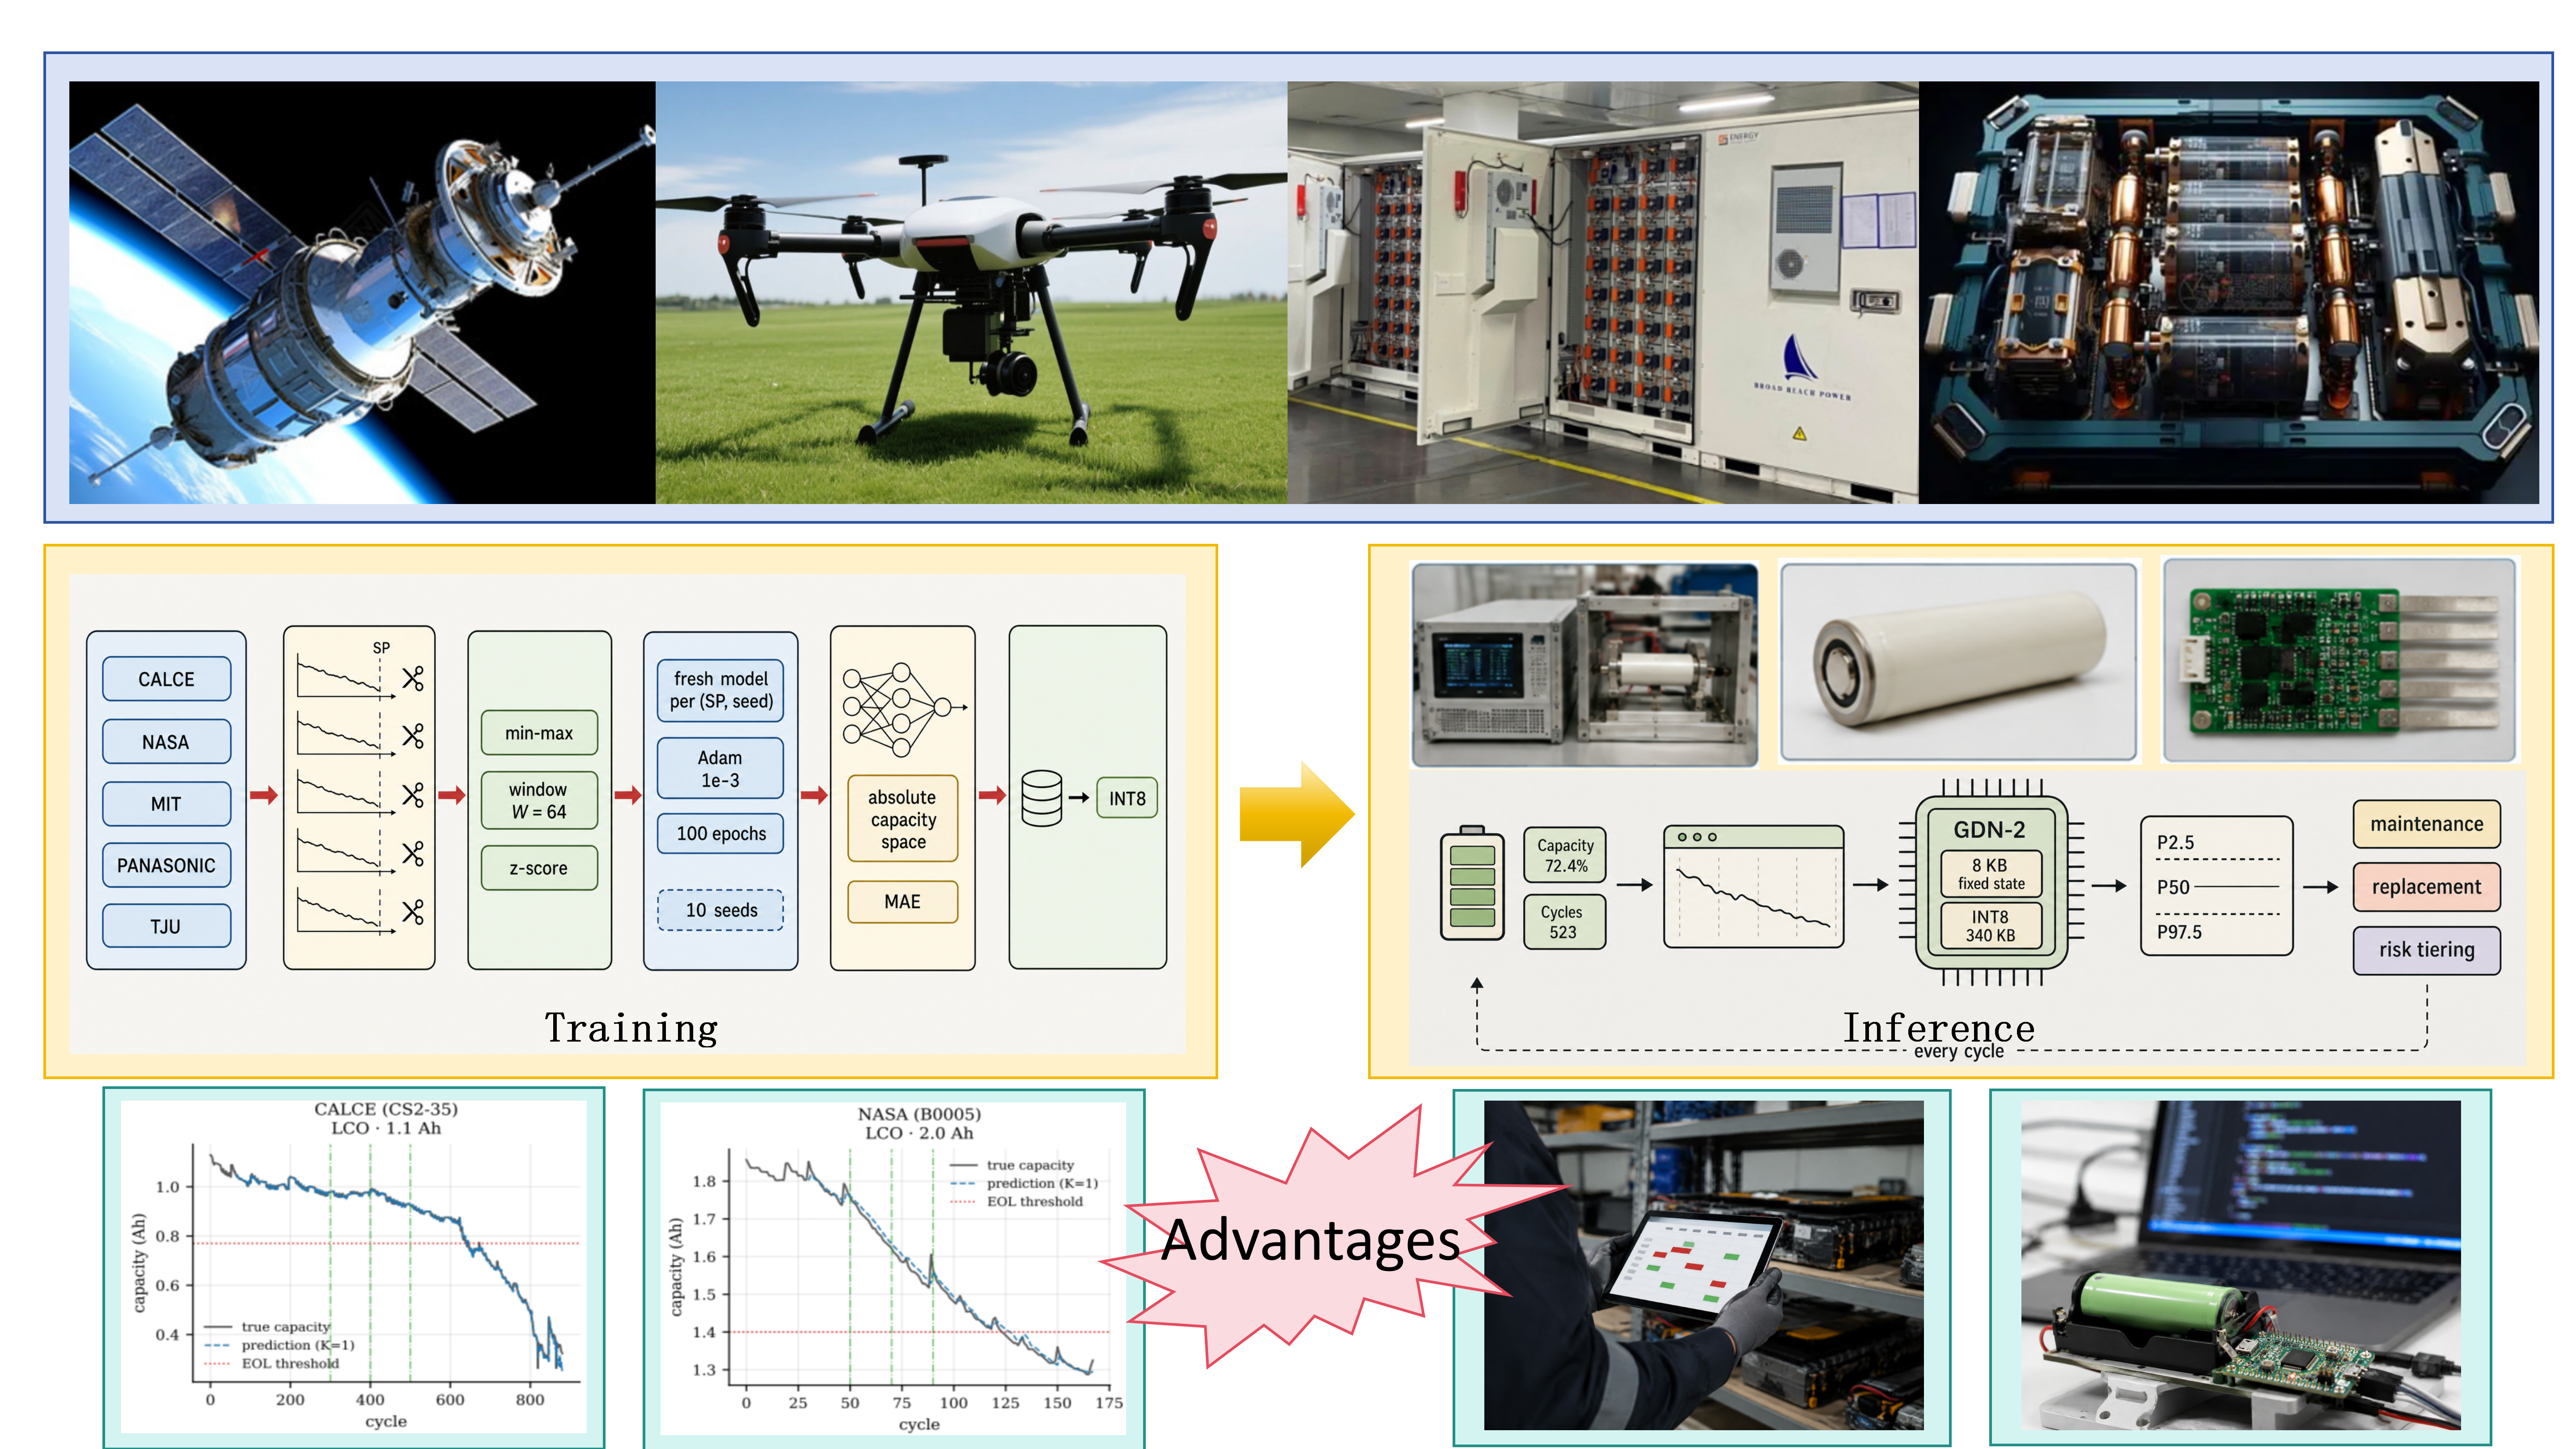
\includegraphics[width=\textwidth]{new_overview.png}
\caption{System overview: the overall pipeline of the proposed
method and an outlook on its application across physical battery
systems with different power and operating profiles: spacecraft
satellites, unmanned aerial vehicles (UAVs), energy-storage battery
cabinets, and power-battery packs. The pipeline starts from public
cycling datasets (CALCE, NASA, MIT, PANASONIC, TJU, GOTION), performs data
preprocessing and trains a fresh model per (dataset, starting point,
seed) under the PatchFormer-consistent protocol, and exports an
INT8-quantized model whose fixed 48\,KB recurrent state does not grow
with the context window, so the window can be lengthened to meet
accuracy requirements without the quadratic attention buffer that
would otherwise dominate SRAM, laying the foundation for on-device
online monitoring.
Application images are illustrative; the experimental validation is
conducted on public laboratory data.}
\label{fig:overview}
\end{figure*}

The technical contributions above map onto the deployment regimes we
target, each stressing a different part of the design rather than
generic monitoring (Figure~\ref{fig:overview}):
no-connectivity edge deployment (spacecraft satellites
and UAV fleets, where physical access and onboard
connectivity budget rule out cloud dependence), risk-aware
scheduling with calibrated intervals (energy-storage battery
cabinets and power-battery packs, where the missed-EOL rate sets
the maintenance window), and regeneration tracking for
non-monotonic field histories. The experimental
validation in this paper is conducted on public laboratory cycling
data and the figure is an application outlook.


The remainder of this paper is organized as follows.
Section~\ref{sec:related} reviews related work.
Section~\ref{sec:method} describes the proposed architecture.
Section~\ref{sec:exp} presents datasets, evaluation protocols, and
experimental results, including ablations, comparison with
PatchFormer, and deployment validation.
Section~\ref{sec:conclusion} concludes the paper.

\section{Related Work}
\label{sec:related}

\subsection{Model-based and traditional machine-learning methods}

Physics-based prognostics build degradation models from electrochemical
dynamics, estimated with filters such as extended Kalman filters
\cite{ref_ekf_yan} and particle filters with electrochemical or empirical state models
\cite{ref_pf_echem,ref_pf_rbf,ref_pf_lui}. These methods encode
mechanistic knowledge but require accurate parameter identification
and struggle with regeneration-rich or heterogeneous degradation.
Traditional machine learning provides a lighter alternative:
support vector machines \cite{ref_svm_klass,ref_svm_patil}, support
vector regression \cite{ref_svr_wang}, and relevance vector machines
\cite{ref_rvm_guo} regress health indicators directly from capacity
or voltage features, yet their fixed kernels cannot easily extrapolate
over the strongly nonlinear EOL-acceleration phase.

\subsection{Deep sequence models for battery prognostics}

Recurrent models were among the first deep approaches to capacity sequences:
LSTM-based predictors \cite{ref_lstm_rul_zhang,ref_lstm_elman_li},
GRU variants \cite{ref_gru_rnn}, and recurrent networks
for RUL \cite{ref_rnn_catelani} capture temporal dynamics but suffer
from long-term dependency limitations. Convolutional hybrids combine
local feature extraction with recurrence, including CNN-BiLSTM
\cite{ref_cnn_bilstm}, TCN-LSTM \cite{ref_tcn_lstm}, and attention
mechanisms \cite{ref_lstm_transformer}. Transformer-based models
\cite{ref_vaswani} brought global attention to battery prognostics:
hybrid CEEMDAN-Transformer-DNN models \cite{ref_ceemdan_trans} and
PatchFormer \cite{ref_patchformer}, which combines dual patch-wise
attention with feature-wise attention. General time-series
transformers evaluated on battery tasks include Autoformer
\cite{ref_autoformer}, FEDformer \cite{ref_fedformer}, iTransformer
\cite{ref_itransformer}, PatchTST \cite{ref_patchtst}, TimesNet
\cite{ref_timesnet}, TimeMixer \cite{ref_timemixer}, PathFormer
\cite{ref_pathformer}, and ModernTCN \cite{ref_moderntcn}. All
attention-based methods share the quadratic-complexity bottleneck
that constrains embedded deployment as the required context grows.
Comprehensive surveys of this
line are given in \cite{ref_lipu_review,ref_he_review}.

\subsection{State space models}

Mamba \cite{ref_mamba} is a selective state space model with
linear-time inference, extensively surveyed in \cite{ref_mamba_survey}
and evaluated for general time-series forecasting in
\cite{ref_samamba_tsf}. For batteries, MambaLithium \cite{ref_mambalithium}
applies a pure Mamba network to SOH/RUL/SOC estimation, and RUL-Mamba
\cite{ref_rulmamba} combines a Mamba encoder with a feature attention
network and a gated residual decoder, reporting state-of-the-art
results on NASA, Oxford, and TJU datasets. While these works emphasize
efficient training and fast inference, their efficiency claims are
based on GPU measurements; none of them validates execution on
embedded hardware, which is the target of the present work.

\subsection{Grey system models}

Grey system theory models degradation using accumulated sequences and
fractional-order operators. Recent work includes grey models with
capacity-regeneration consideration \cite{ref_grey_hybrid}, adaptive
weighted fractional-order reverse accumulation for SOH
\cite{ref_grey_frac}, fractional-order heuristic models for PEMFC
prognostics \cite{ref_grey_pemfc}, self-adaptive grey neural networks
for real-time PEMFC degradation \cite{ref_grey_nn}, grey Kalman
filtering for SOC estimation \cite{ref_grey_kalman}, and grey
iterative modeling for battery health management \cite{ref_grey_iter}.
These methods are lightweight and interpretable but rely on
hand-crafted model forms that must be re-specified for each battery
chemistry and operating regime.

\subsection{Physics-informed battery modeling}

Physics-informed neural networks (PINNs) embed degradation physics
into the learning objective. Wang et al.\ \cite{ref_wang_pinn}
proposed a physics-informed network for stable degradation modeling,
and PiDDM \cite{ref_piddm} incorporates Arrhenius degradation kinetics
into the training objective, reporting improved extrapolation at the
end of life. Our systematic injection-route study (Section
\ref{sec:exp-phys}) revisits this question for a sequence model that
already ingests the capacity trajectory: objective regularization,
input feature concatenation, and structural heads all fail: the
per-window z-score target space is structurally incompatible with
monotone predictors, and the features are redundant with capacity
history. The remaining route is a degradation-rate head driven by
measured internal resistance, trained in absolute capacity space
(Section~\ref{sec:rate-head}).

\subsection{Linear attention and recurrent mixing}

Linear attention and state space models share the recurrent-state
view, and the two families are sometimes presented as one; we keep
them apart because the battery-SSM literature above frames
efficiency as a GPU concern, while the delta-rule family below is
the technical lineage of our backbone. Linear attention replaces the softmax attention map with a recurrent
matrix state, achieving $O(N)$ complexity. Gated DeltaNet
\cite{ref_gdn} combined the delta rule with learned gating, and
Gated DeltaNet-2 (GDN-2) \cite{ref_gdn2} decoupled channel-wise erase
and write gates, improving long-context retrieval in language
modeling. To our knowledge, the present work is the first to report
floating-point-accurate MCU deployment of a linear-attention battery model.

Stepping back from individual architectures, the surveyed literature
answers one question, which model is most accurate on public cycling
data, while leaving the questions that decide operational adoption
largely open. First, accuracy has been demonstrated only on
server-class hardware: none of the battery-specific models above
reports a deployment path onto the microcontrollers that production
BMS firmware actually runs on, so operators must either pay for
cloud connectivity or accept simpler on-device estimators. Second,
forecasts are evaluated as point trajectories, yet the operational
consumer of a forecast is a maintenance schedule, which requires an
explicit statement of risk; few works report calibrated intervals
suitable for scheduling. Third, evaluations are confined to clean
laboratory data: the end-of-life acceleration tail and the
corrupted-sensor regimes, where field decisions concentrate, are
rarely tested, so reported accuracy says little about how a
predictor will behave in deployment. DeltaCycle is designed around
these three operational gaps rather than around a single benchmark
number.

\section{Method}
\label{sec:method}

\subsection{Problem formulation and input design}
\label{sec:formulation}

We formulate battery prognostics as a sliding-window capacity
forecasting problem. Let $c_t$ denote the measured capacity at cycle
$t$. Given a fixed-length input window
$\mathbf{X}_{t} = [c_{t-W+1}, \ldots, c_t]$ of historical capacity,
the model predicts future capacity values. The main model
deliberately consumes capacity only, for a deployment-driven
reason: at inference the future values of voltage, current,
temperature and internal resistance are unavailable, so a model that
consumes them cannot predict to the end of life without information
leakage. Capacity is the only health indicator that is both
measurable online and sufficient on its own for long-horizon
prediction. The physics-consistent extension of
Section~\ref{sec:rate-head} additionally consumes the per-cycle
measured internal resistance, a quantity the BMS records in
situ and that is available at inference without future information, so the
extension remains deployable under the same constraint.

\subsection{Gated DeltaNet-2 backbone}
\label{sec:gdn2}

The backbone is Gated DeltaNet-2 (GDN-2) \cite{ref_gdn2}, a
recurrent linear attention layer with channel-wise erase and write
gates. GDN-2 generalizes Gated DeltaNet \cite{ref_gdn}, which ties
erasing and writing to a single scalar gate, by moving each to its own
channel-wise gate: erase on the key axis, write on the value axis. It
recovers Gated DeltaNet exactly when both gates and the decay
collapse to scalars. For one head with key dimension $d_k$ and value dimension
$d_v$, the recurrence is
\begin{equation}
\label{eq:gdn2}
\mathbf{S}_t \;=\; \left( \mathbf{I} - \mathbf{k}_t(\mathbf{b}_t
\odot \mathbf{k}_t)^{\top} \right)
\operatorname{diag}(\boldsymbol{\alpha}_t)\, \mathbf{S}_{t-1}
\;+\; \mathbf{k}_t(\mathbf{w}_t \odot \mathbf{v}_t)^{\top},
\end{equation}
\begin{equation}
\label{eq:readout}
\mathbf{o}_t \;=\; \mathbf{S}_t^{\top}\mathbf{q}_t,
\end{equation}
where $\mathbf{q}_t,\mathbf{k}_t \in \mathbb{R}^{d_k}$ and
$\mathbf{v}_t \in \mathbb{R}^{d_v}$ are query, key, and value vectors;
$\mathbf{b}_t \in \mathbb{R}^{d_k}$ is the channel-wise erase gate and
$\mathbf{w}_t \in \mathbb{R}^{d_v}$ the channel-wise write gate, both
bounded to $[0,1]$ by a sigmoid; and
$\boldsymbol{\alpha}_t = \exp(\mathbf{g}_t)$ is the channel-wise decay
with
\begin{equation}
\mathbf{g}_t \;=\; -A_{\log}\cdot
\operatorname{softplus}\!\big( f(\mathbf{x}_t) + \mathbf{d}_t \big),
\end{equation}
where $\mathbf{x}_t$ is the input token at position $t$ (the embedded
capacity, or the branch's hidden representation after the first
layer), $A_{\log}$ is a per-head log-rate, $f(\cdot)$ a two-layer
projection, and $\mathbf{d}_t$ a per-channel bias. The state
$\mathbf{S}_t \in \mathbb{R}^{d_k \times d_v}$ is fixed-size and
updated incrementally, yielding $O(N)$ scan complexity with
constant memory. With $H$ heads, $d_k=16$, and $d_v=32$, the total
state is $H \cdot d_k \cdot d_v \cdot 4$ bytes $= 8$\,KB per layer.
During a window scan the state is updated incrementally: each new
cycle erases part of the old memory (via $\mathbf{b}_t$) and writes
new information (via $\mathbf{w}_t$), so the fixed-size matrix acts
as an adaptive compression of the degradation history rather than a
static buffer. Decoupling the two axes is what makes that compression
useful for a capacity series, which mixes a slow global fade that
should persist in the state with regeneration excursions that should
not: a single scalar gate can only trade the two against each other
uniformly across all channels, whereas separate erase and write gates
let the layer drop a stale association without also suppressing the
channels that carry the trend.

\subsection{Multi-scale branches with per-layer cross-scale exchange}
\label{sec:multiscale}

Figure~\ref{fig:arch} shows the multi-scale encoder
together with the per-layer cross-scale exchange submodule (bottom,
light-green box), and Figure~\ref{fig:gdn2} details the internal
recurrence of one GDN-2 block.

\begin{figure*}[!t]
\centering
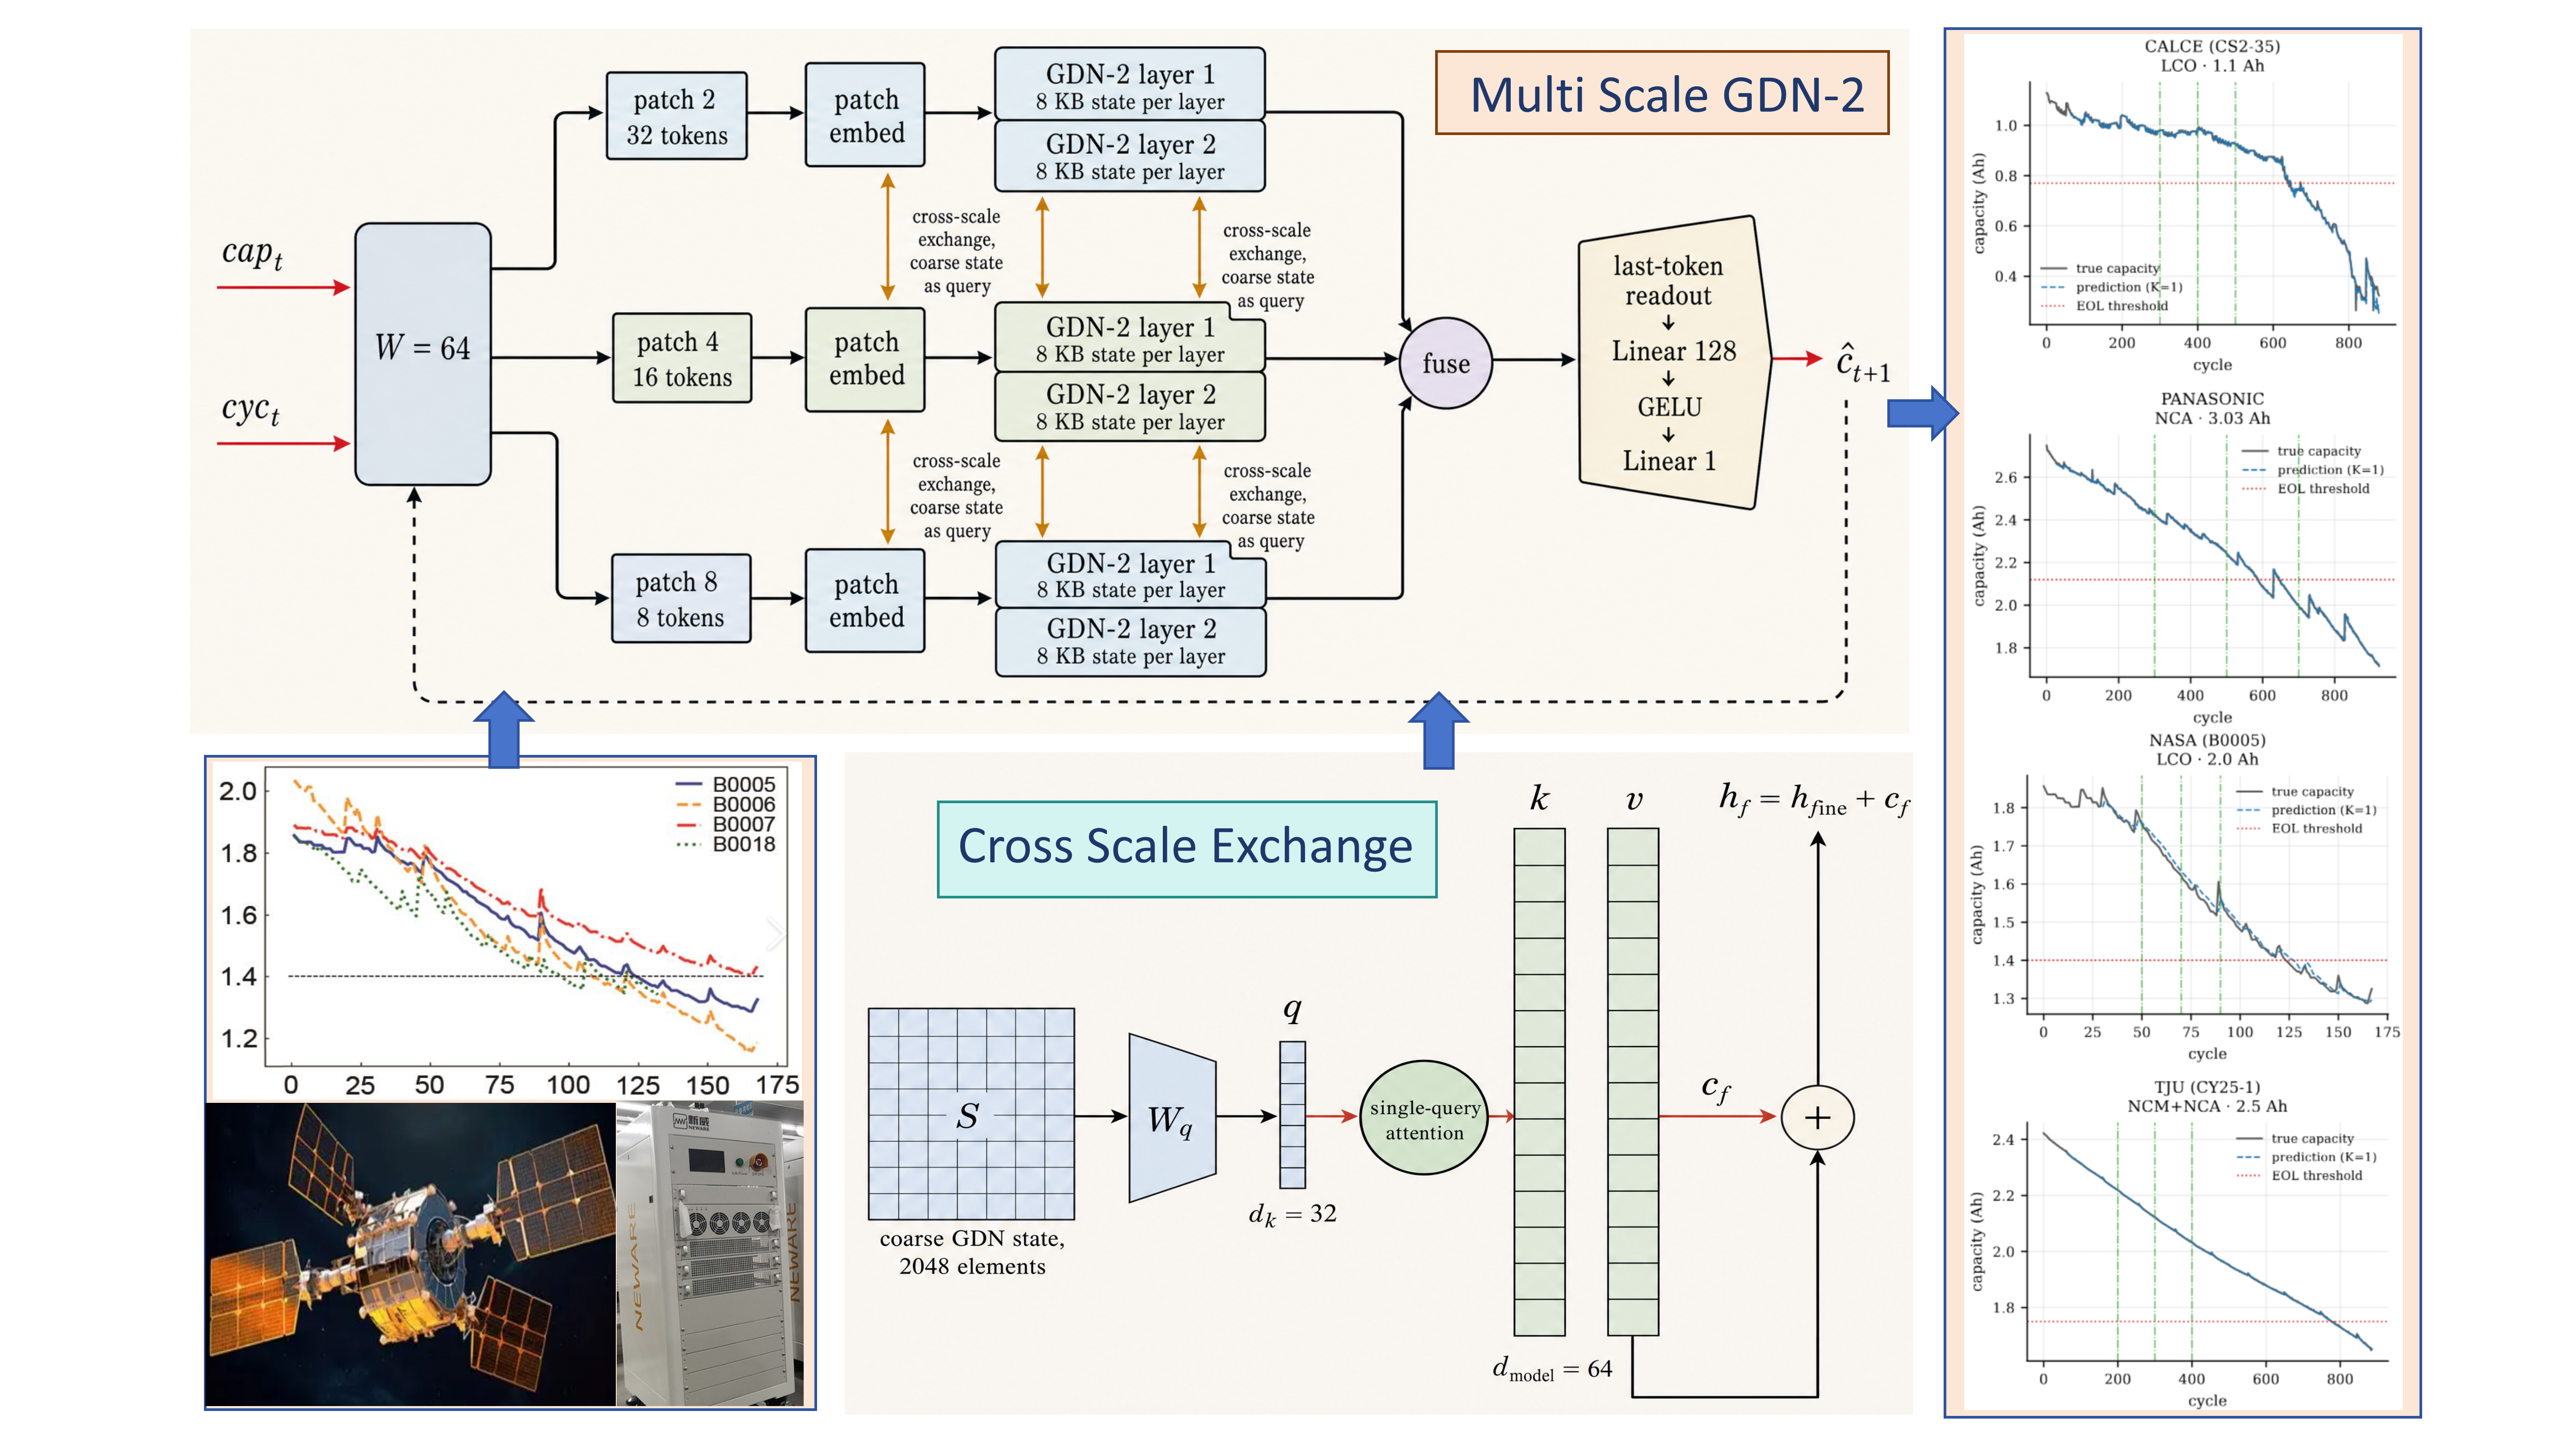
\includegraphics[width=\textwidth]{new_modelarch.png}
\caption{Multi-scale GDN-2 architecture and cross-scale exchange
submodule. Top: the fixed window of $W{=}64$ capacity cycles (the
tokens $cap_t$; $cyc_t$ denotes the cycle index) is encoded in
parallel at three scales (patch 2/4/8, 32/16/8 tokens), embedded
per scale, and passed through two GDN-2 layers per branch ($8$\,KB
fixed state per layer); the three branches exchange multi-scale
information through the per-layer cross-scale exchange (orange
arrows, coarse state as query), fuse at the $fuse$ node, and emit
the next-cycle capacity prediction
$\hat{c}_{t+1}$ via the last-token readout (Linear\,128 $\to$ GELU
$\to$ Linear\,1). Bottom (light-green box): the cross-scale exchange
submodule maps the coarse state $S$ (2048 elements) to a single
query $q$ ($d_q{=}32$) via $W_q$; single-query attention interacts
$q$ with the fine/mid branch keys and values ($k, v$,
$d_{\text{model}}{=}64$) to produce the context $c_f$, added to the
fused state: $h_f = h_{\text{fuse}} + c_f$.}
\label{fig:arch}
\end{figure*}

\begin{figure}[htbp]
\centering
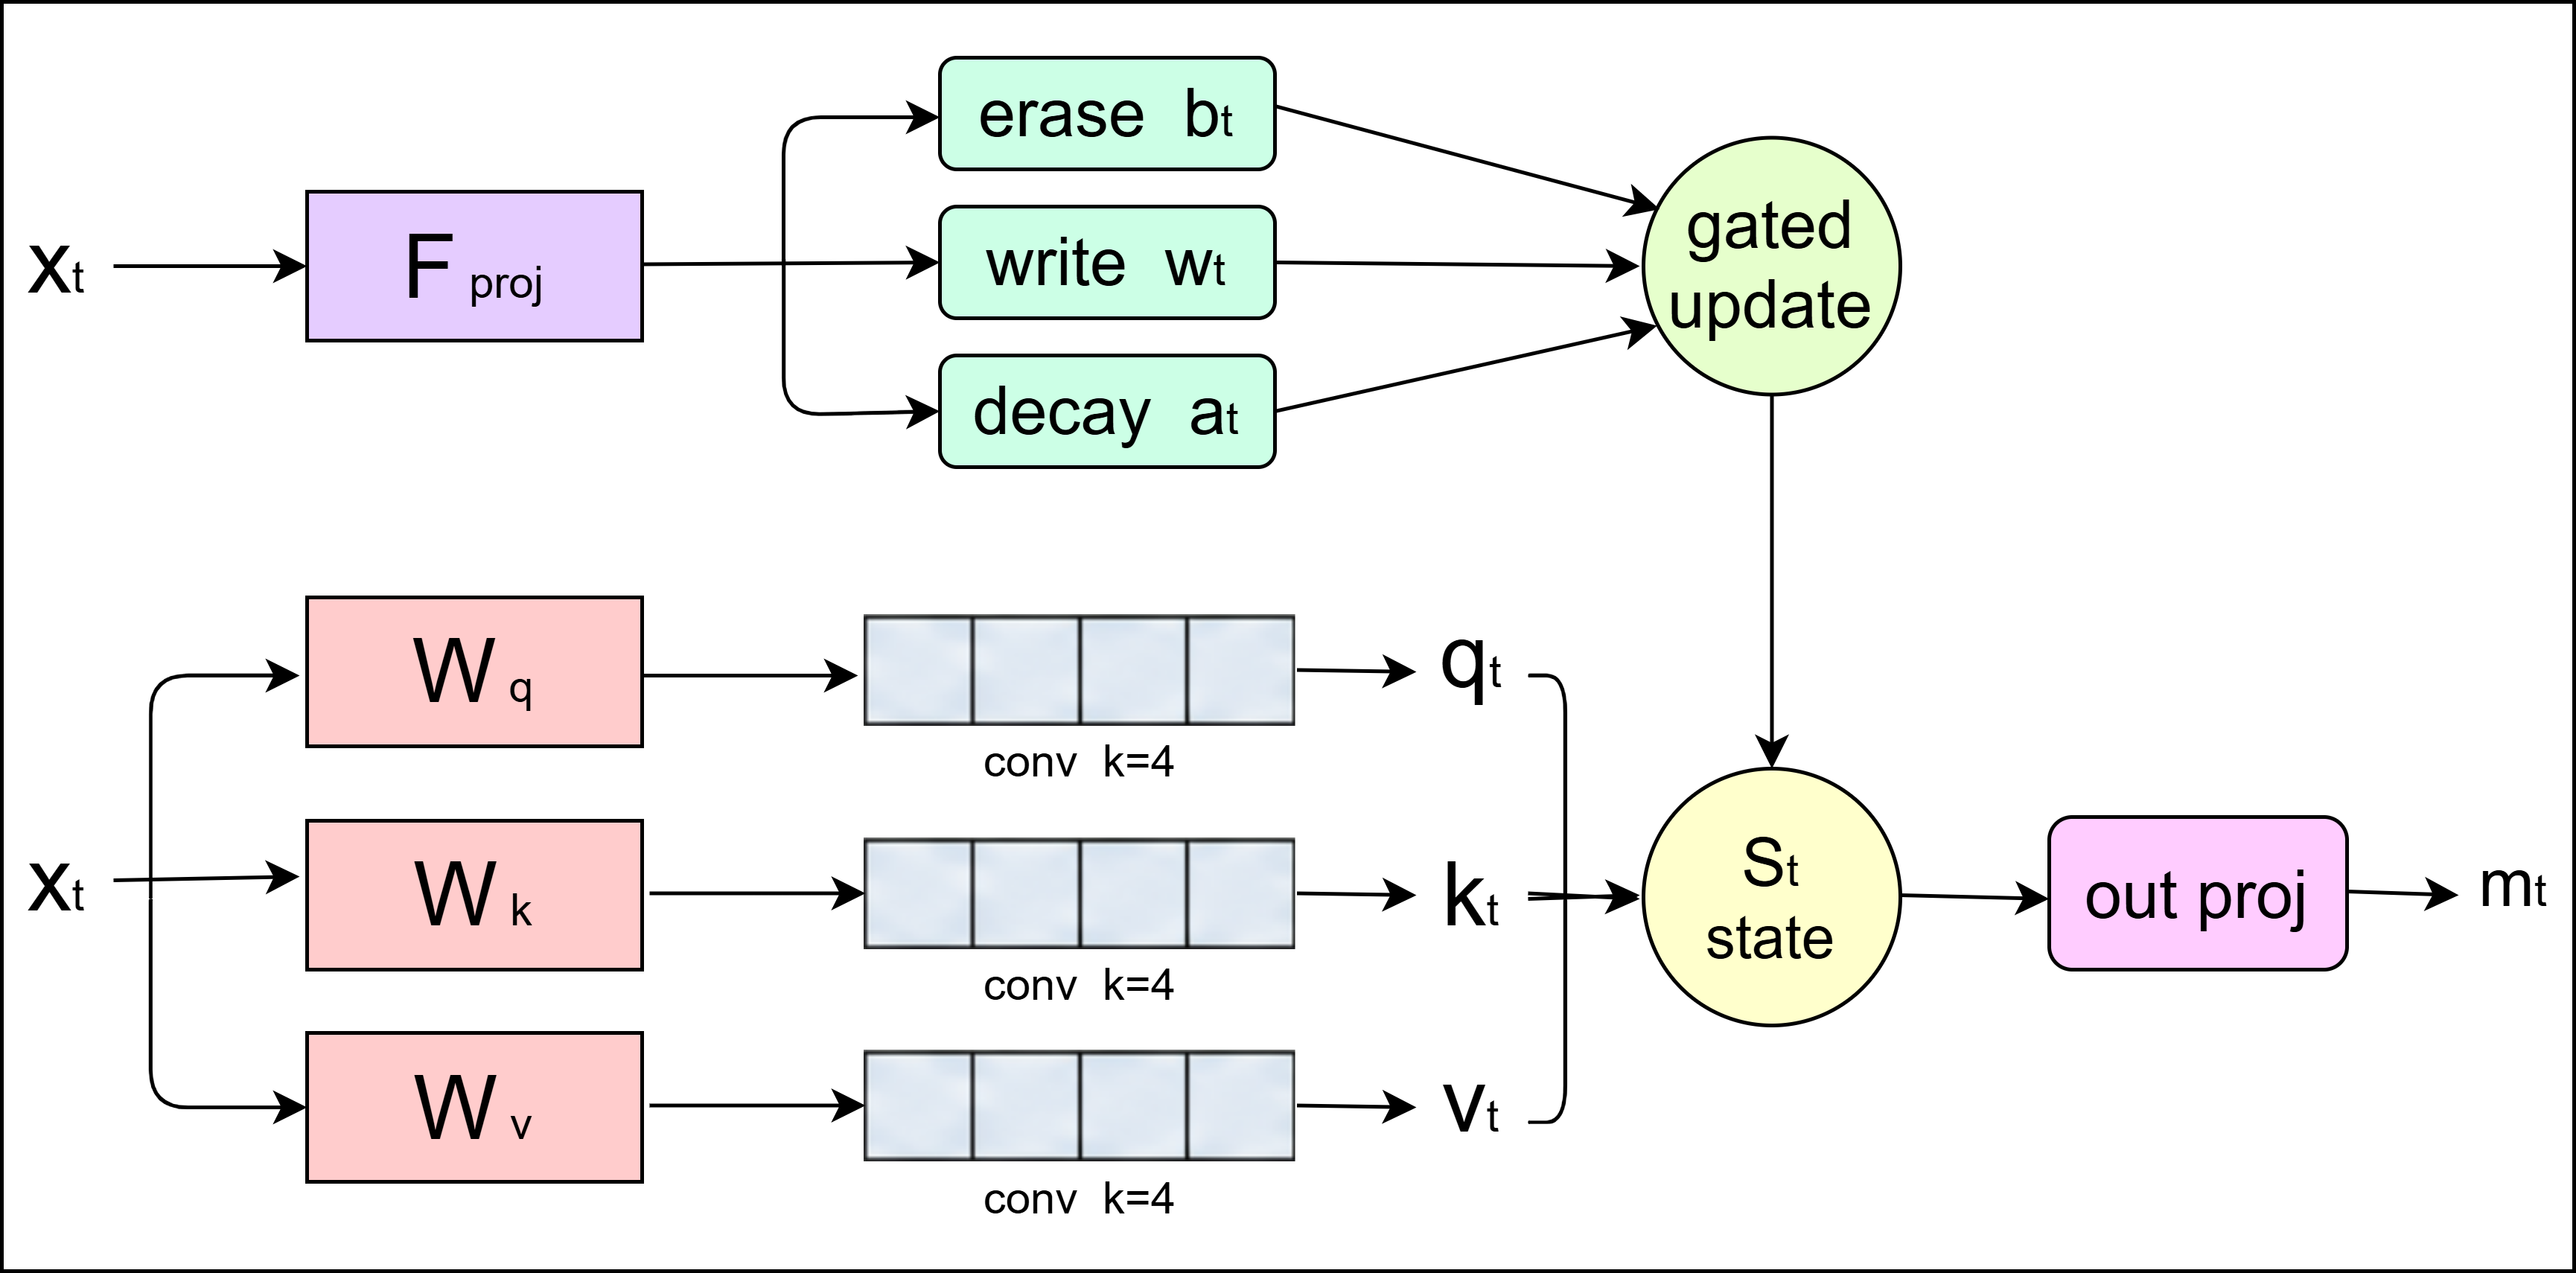
\includegraphics[width=\linewidth]{fig_gdn2_flow}
\caption{One GDN-2 block. The input token $x_t$ is projected to
queries/keys/values ($W_q$: $64\to64$, $W_k$: $64\to64$,
$W_v$: $64\to128$), each through a causal 1-D convolution
(kernel $k{=}4$, $L2$-normalized for $q$ and $k$), while a shared
projection $F_{\mathrm{proj}}$ generates the erase
($\mathbf{b}_t$, sigmoid), write ($\mathbf{w}_t$, sigmoid) and
per-channel decay ($\boldsymbol{\alpha}_t = \exp(g)$) gates; the
gated update produces the fixed-size state
$\mathbf{S}_t$ ($4\times16\times32$ elements $= 8$\,KB, zero
growth), and the output
$\mathbf{o}_t = \mathbf{S}_t^{\top}\mathbf{q}_t \to$ Linear
$128\to64 \to$ RMSNorm.
}
\label{fig:gdn2}
\end{figure}

Battery degradation operates across multiple temporal scales: short
regeneration events, mid-range knee-point transitions, and the
long-term monotonic envelope. We encode these with three parallel
branches using patch sizes $P \in \{2,4,8\}$. Each branch projects its
patched input to a common $d_{\text{model}}=64$ embedding and applies
two GDN-2 layers. Each branch scans at its own token count (32, 16 and
8 for patch sizes 2, 4 and 8), and the branches are aligned to the
longest only before an exchange, since aligning first would scan the
wrong sequence length. The two length operations differ: aligning tiles
the whole sequence to the longest token count
($[a,b,c]\mapsto[a,b,c,a,b,c]$), whereas restoring a branch to the full
input length repeats each token ($[a,b,c]\mapsto[a,a,b,b,c,c]$).
After every GDN layer, branches exchange
information through a stage-query mechanism: the coarse branch's
GDN-2 state, which compresses the degradation history and acts as a
stage indicator, is projected to a single query, and the fine and
mid branch sequences provide keys and values. For branch
$\mathbf{h}_a$ with the coarse state $\mathbf{S}_c$,
\begin{equation}
\label{eq:stagequery}
\mathbf{q} \;=\; \mathbf{W}_q \operatorname{vec}(\mathbf{S}_c),
\qquad
\mathbf{h}_a' \;=\; \mathbf{h}_a \;+\;
\sum_{t} \frac{\exp\!\big(\mathbf{k}_t^{\top}\mathbf{q}/\sqrt{d_k}\big)}
{\sum_{s} \exp\!\big(\mathbf{k}_s^{\top}\mathbf{q}/\sqrt{d_k}\big)}
\,\mathbf{v}_t,
\end{equation}
where $\mathbf{k}_t = \mathbf{W}_k \mathbf{h}_a[t]$ and
$\mathbf{v}_t = \mathbf{W}_v \mathbf{h}_a[t]$, and the summation is a
single-query linear-attention readout with $O(L)$ cost per layer.
The exchange is additive (residual, no gating) and applied
per layer. A parameter-matched ablation
(Section~\ref{sec:ablation}) isolates its contribution: with both arms
grown to the same parameter count on PANASONIC, the exchange lowers
per-SP MAE by $5.7\,\%$ on average ($p=0.014$), winning $22$ of the $30$
(starting point, seed) pairs.

An interpretability analysis (Section \ref{sec:exp-phys}) reveals that
the coarse branch (patch 8) spontaneously encodes the degradation
stage: its pooled representation is $93.2\%$ linearly separable into
early/mid/late life stages on the PANASONIC dataset ($2.9\times$
chance), providing stage-aware state awareness at no additional
supervision cost.

\subsection{Physics-consistent extension: the rate head}
\label{sec:rate-head}

The main architecture of Section~\ref{sec:multiscale} is trained
purely data-driven under the baseline-consistent per-window protocol.
Here we present a physics-consistent extension whose design is the
outcome of a systematic injection-route study (Section
\ref{sec:exp-phys}): a degradation-rate head driven by a measured
physical feature. Lithium-ion capacity fade is governed by
thermally activated processes (solid-electrolyte-interface growth,
loss of lithium inventory and active-material loss), and internal
resistance (IR) is a direct, independently measured observable of
these aging processes that rises as the cell degrades. We therefore
decompose the per-cycle decay rate into a learned component and a
physics-feature component:
\begin{equation}
\label{eq:rate_head}
r \;=\; \operatorname{softplus}(\mathbf{w}^{\top}\mathbf{h})
\;+\; \operatorname{softplus}(\gamma)\cdot \mathrm{IR}_{\text{last}},
\qquad
\hat{c}_{t+1} \;=\; c_t - r,
\end{equation}
where $\mathbf{h}$ is the last-token GDN state, $c_t$ the current
capacity, $\mathrm{IR}_{\text{last}}$ the measured internal
resistance at the current cycle, and $\gamma$ a learned scalar. The
softplus makes the coefficient $\operatorname{softplus}(\gamma)$
non-negative, so internal-resistance growth can only \emph{accelerate}
decay, never decelerate it. This is the physical direction of SEI-driven
aging. The formulation is structurally monotonic
($\hat{c}_{t+1} \le c_t$) and therefore cannot emit nonphysical
regeneration artifacts by construction.

The rate head is trained in \emph{absolute} capacity space
($\mathcal{L} = \operatorname{MAE}(\hat{c}, c)$) rather than the
per-window z-score protocol: z-score targets include positive values
(plateau segments where the next observation lies above the window
mean) that a monotone predictor can never produce, so the constraint
is unsatisfiable in that space; the absolute-space objective removes
the sign conflict. A control experiment confirms the mechanism, not
the objective, is responsible for the gain: over ten seeds a free head
trained in absolute space reaches MAE $0.0089\pm0.0058$ (worse than
the z-score free head at $0.0065\pm0.0003$), while the rate head
reaches $0.00424\pm0.00002$. The extension
further improves the unseen-tail extrapolation ($R^2$ $0.775$ vs
$0.374$) and robustness to corrupted inputs (Section
\ref{sec:exp-phys}).

\subsection{Readout and training protocol}
\label{sec:readout}

After the multi-scale encoder, the fused last-token representation
$\mathbf{h}_{t}$ is passed through a readout
\begin{equation}
\label{eq:head}
\hat{c}_{t+1}
\;=\; \operatorname{Head}(\mathbf{h}_t)
\;=\; \mathbf{W}_2\, \mathrm{GELU}(\mathbf{W}_1 \mathbf{h}_t),
\end{equation}
with $d = 3 \cdot d_{\text{model}} = 192$ the dimension of the fused
last-token representation (concatenation of the three branches),
$\mathbf{W}_1 \in \mathbb{R}^{128 \times d}$ and
$\mathbf{W}_2 \in \mathbb{R}^{1 \times 128}$. The model is trained
with the per-window z-score target protocol of PatchFormer and
RUL-Mamba for baseline comparability: the input window is normalized
globally with training-cell min--max statistics, the target is
$(c_{t+1} - \bar{c})/\sigma_c$ with window statistics
$(\bar{c}, \sigma_c)$, and predictions are de-normalized with the
same window statistics at evaluation.

\subsection{Uncertainty quantification with conformal calibration}
\label{sec:quantile}

Safety-critical BMS decisions require not only a point estimate of
the health state but a calibrated interval, e.g., ``the cell will
cross the EOL threshold within 30--50 cycles with 95\% confidence''.
To provide this without the cost of an ensemble, the readout head
outputs three quantiles per forward pass,
$q \in \{0.025, 0.5, 0.975\}$ (P2.5, the median P50, and P97.5),
bounding a central 95\% interval. The head is trained
with the pinball (quantile) loss
\begin{equation}
\begin{split}
\mathcal{L}_{\text{pin}} &=
\frac{1}{N}\sum_{i}\sum_{q \in \{0.025,0.5,0.975\}}
\rho_q\!\left( c_i - \hat{c}_i^{(q)} \right), \\
&\quad \rho_q(u) = \max(q u, (q-1) u),
\end{split}
\end{equation}
where $c_i$ is the observed capacity, $\hat{c}_i^{(q)}$ is the
predicted $q$-quantile, and the pinball function $\rho_q$ penalizes
under-prediction (when $\hat{c}^{(q)} > c$) by a factor $q$ and
over-prediction by $1-q$, so that the minimizer is the conditional
$q$-quantile. Because a lower capacity trajectory crosses the EOL
threshold earlier, P2.5 yields the \emph{earliest} plausible EOL
crossing and P97.5 the \emph{latest}; the P2.5--P97.5 crossing
window is therefore a safety-relevant interval (the pessimistic
bound drives maintenance scheduling).

Quantile regression alone is known to be miscalibrated under
distribution shift. We therefore apply \emph{conformalized quantile
regression} (CQR): a held-out calibration cell provides conformity
scores $s_i = \max(\hat{c}_i^{\text{lo}} - c_i,\; c_i -
\hat{c}_i^{\text{hi}})$, and the deployed interval is inflated by
$q_{\text{adj}}$, the $(1-\alpha)(1+1/n)$ empirical quantile of the
scores, where $\alpha = 0.05$ and $n$ is the calibration size.
Calibration and coverage results are reported in
Section~\ref{sec:conf}. The entire UQ mechanism costs one forward
pass and two scalars at deployment: no ensemble, no MC sampling.


\section{Experiments}
\label{sec:exp}

\subsection{Datasets}
\label{sec:datasets}

We evaluate on six public battery degradation datasets spanning
different chemistries, capacities, and degradation behaviors
(Table~\ref{tab:datasets}): CALCE (LCO, rated 1.1\,Ah), NASA
\cite{ref_nasa_data} (LCO, 2.0\,Ah), MIT/Stanford \cite{ref_severson}
(LFP, 124 cells), PANASONIC (NCA, 3.03\,Ah), TJU (NCM+NCA,
2.5\,Ah), and GOTION (LFP large-format, 27\,Ah). End-of-life (EOL) thresholds follow rated
capacity times convention: 70\% for small cells and 80\% for
large-format cells; for the MIT/Stanford set we follow the 80\% convention of its
original publications \cite{ref_severson}. For MIT we use a 10-cell subset (8 training, 2 test) for this study.
All models use pure capacity input; internal resistance is used only
as an auxiliary input of the physics-extension rate head
(Section~\ref{sec:rate-head}).

\begin{table}[htbp]
\centering
\caption{Dataset overview.}
\label{tab:datasets}
\tiny
\begin{tabular}{lccccc}
\toprule
Dataset & Chemistry & Rated & Cells & EOL (Ah) & Role \\
\midrule
CALCE & LCO & 1.1 Ah & 4 & 0.77 & primary, physics (IR) \\
NASA & LCO & 2.0 Ah & 4 & 1.40 & short-history \\
MIT & LFP & 1.07 Ah & 10$^{\ast}$ & 0.86 & cross-battery \\
PANASONIC & NCA & 3.03 Ah & 3 & 2.12 & regeneration \\
TJU & NCM+NCA & 2.5 Ah & 3 & 1.75 & long-cycle \\
GOTION & LFP (large-format) & 27 Ah & 3 & 21.60 & large-format fleet \\
\bottomrule
\multicolumn{6}{@{}p{\dimexpr\columnwidth-6pt\relax}@{}}{\footnotesize
$^{\ast}$MIT results use a 10-cell subset (8 training, 2 test); every other
dataset uses all of its cells.}\\
\end{tabular}
\end{table}

\subsection{Evaluation protocol}
\label{sec:protocol}

Following the standard protocol in PatchFormer \cite{ref_patchformer}
and RUL-Mamba \cite{ref_rulmamba}, we report trajectory
metrics per starting point (SP): R\textsuperscript{2}, MAE (mean absolute error),
RMSE (root mean squared error), and AE. Let TRUL be the true
remaining useful life in cycles at an SP (cycles from the SP to the
true EOL crossing), PRUL is the predicted RUL from the first threshold
crossing of the predicted capacity sequence (taken at its first occurrence, so
a single-sample dip counts even where the prediction recovers on the next
step), and AE $= |\text{TRUL} - \text{PRUL}|$ is the absolute RUL error in
cycles.

\emph{Training configuration.} All models use Adam (learning rate
$1\times10^{-3}$, batch size 64) for 100 epochs with a window of
$W{=}64$ cycles ($W{=}30$ for NASA, PANASONIC and GOTION, matching the
window convention of the baseline literature). These settings were
fixed during the ablation stage and held constant across datasets,
seeds, and model variants: no per-dataset or per-variant tuning is
applied to the reported results, so every variant compared in
Sections~\ref{sec:ablation}--\ref{sec:exp-phys} shares the same optimizer
budget. A sensitivity note on these choices is in
Section~\ref{sec:limitations}.
The main results (Table~\ref{tab:tableA}) additionally follow the
per-SP training protocol of PatchFormer. For each combination of dataset, prediction Start Point (SP), 
and random seed, a separate model with randomly initialized weights is trained from scratch, 
with no pre-trained weights or cross-set parameter reuse allowed. We use ten seeds per
SP (1--10), so each table cell aggregates ten independently trained
models. The ablation studies (Section~\ref{sec:ablation}) use the
same optimizer budget with ten seeds. The physics extension is
reported over the same ten seeds for its head, extrapolation, and
robustness studies, and the uncertainty study uses the ten-seed
full-data training described above (coverage
$93.5\%\pm0.9\%$).

\subsection{Main results}
\label{sec:main}

Figure~\ref{fig:traj} shows representative SOH trajectories with
sliding-window predictions for one cell of each dataset;
Table~\ref{tab:tableA} reports the full per-SP results. The six datasets span distinct degradation regimes 
and operational scenarios. We present each as a standalone case study in the sections below: 
each case concludes with a discussion of the practical implications of our experimental results, 
as well as a benchmark comparison against state-of-the-art (SOTA) results reported on the same dataset.

\begin{figure*}[!t]
\centering
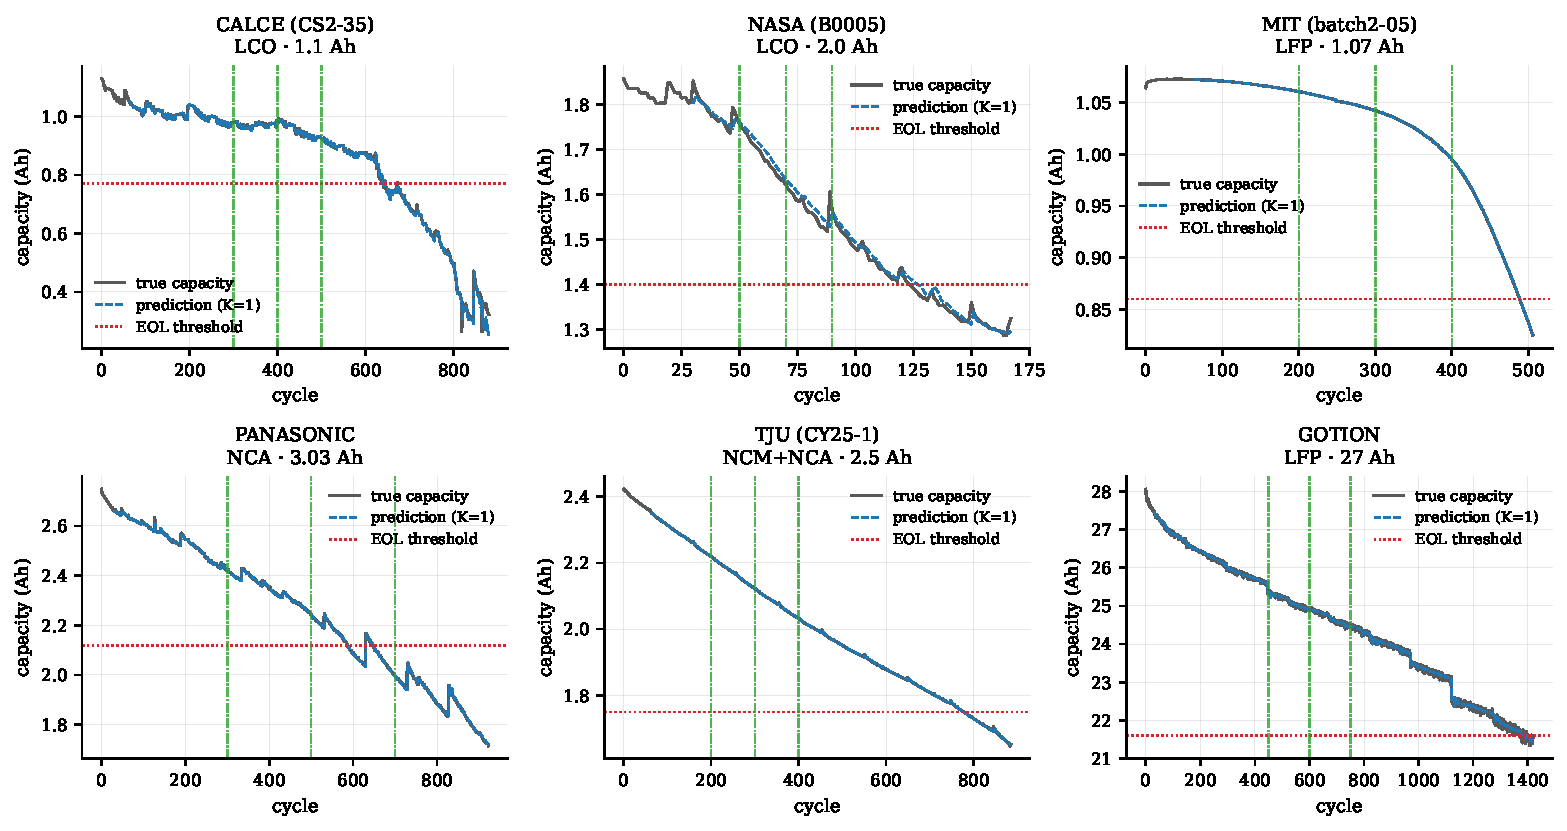
\includegraphics[width=\textwidth]{fig_traj}
\caption{Capacity prediction on one test cell per
dataset. Green dashed lines mark the starting points (SPs); red
dotted lines mark the EOL thresholds.}
\label{fig:traj}
\end{figure*}


Figure~\ref{fig:compare} shows our model ranks first (mean per-SP MAE) on PANASONIC, TJU, GOTION and MIT,
and second on NASA and CALCE---top-2 on all six datasets and
ahead of every generic time-series transformer.

\begin{figure*}[!t]
\centering

\includegraphics[width=\textwidth]{fig_compare}
\caption{Per-SP trajectory MAE of the compared methods on all six
datasets, averaged over the three SPs (log scale). Green: Ours; blue:
PatchFormer/RUL-Mamba; gray: other baselines.}
\label{fig:compare}
\end{figure*}

\begin{table}[htbp]
\centering
\caption{Per-SP trajectory results, mean $\pm$ std
over ten seeds (1--10) per SP under the PatchFormer-consistent
per-SP protocol (a fresh model per (SP, seed)).}
\label{tab:tableA}
\scriptsize
\setlength{\tabcolsep}{1pt}
\begin{tabular}{lr rrrrr}
\toprule
Dataset & SP & TRUL & MAE & RMSE & R\textsuperscript{2} & AE \\
\midrule
CALCE & 300 & 339 & 0.0065$\pm$0.0007 & 0.0145$\pm$0.0013 & 0.9951$\pm$0.0008 & 3.2 \\
  & 400 & 239 & 0.0077$\pm$0.0010 & 0.0169$\pm$0.0019 & 0.9933$\pm$0.0015 & 2.5 \\
  & 500 & 139 & 0.0091$\pm$0.0016 & 0.0194$\pm$0.0028 & 0.9898$\pm$0.0030 & 2.4 \\
NASA & 50 & 73 & 0.0086$\pm$0.0016 & 0.0128$\pm$0.0011 & 0.9908$\pm$0.0018 & 0.9 \\
  & 70 & 53 & 0.0078$\pm$0.0008 & 0.0130$\pm$0.0004 & 0.9822$\pm$0.0011 & 0.4 \\
  & 90 & 33 & 0.0071$\pm$0.0008 & 0.0101$\pm$0.0010 & 0.9804$\pm$0.0036 & 0.5 \\
PANASONIC & 300 & 287 & 0.0038$\pm$0.0003 & 0.0098$\pm$0.0001 & 0.9976$\pm$0.0001 & 0.8 \\
  & 400 & 187 & 0.0037$\pm$0.0002 & 0.0103$\pm$0.0001 & 0.9965$\pm$0.0001 & 0.8 \\
  & 500 & 87 & 0.0041$\pm$0.0003 & 0.0113$\pm$0.0003 & 0.9936$\pm$0.0003 & 0.9 \\
TJU & 200 & 577 & 0.0010$\pm$0.0002 & 0.0015$\pm$0.0001 & 0.9999$\pm$0.0000 & 0.2 \\
  & 300 & 477 & 0.0011$\pm$0.0002 & 0.0016$\pm$0.0002 & 0.9998$\pm$0.0000 & 0.9 \\
  & 400 & 377 & 0.0014$\pm$0.0003 & 0.0020$\pm$0.0004 & 0.9996$\pm$0.0001 & 1.6 \\
MIT & 200 & 406 & 0.0005$\pm$0.0002 & 0.0008$\pm$0.0003 & 0.9998$\pm$0.0002 & 0.9 \\
  & 300 & 306 & 0.0007$\pm$0.0002 & 0.0009$\pm$0.0004 & 0.9997$\pm$0.0004 & 0.9 \\
  & 400 & 206 & 0.0008$\pm$0.0004 & 0.0010$\pm$0.0004 & 0.9995$\pm$0.0004 & 1.1 \\
GOTION & 450 & 921 & 0.0473$\pm$0.0006 & 0.0645$\pm$0.0013 & 0.9970$\pm$0.0001 & 18.2 \\
  & 600 & 771 & 0.0518$\pm$0.0019 & 0.0697$\pm$0.0026 & 0.9958$\pm$0.0003 & 10.7 \\
  & 750 & 621 & 0.0550$\pm$0.0006 & 0.0735$\pm$0.0019 & 0.9938$\pm$0.0003 & 15.1 \\
\midrule
\multicolumn{7}{l}{\emph{Average across all SPs and seeds: AE = 3.4 cycles, R\textsuperscript{2} = 0.9947.}} \\
\bottomrule
\end{tabular}
\end{table}

\begin{table*}[!t]
\centering
\caption{Comparison with reference baselines on all six
published-comparison datasets. MAE in Ah; each
dataset's starting points are listed under its name; bold marks the
best value in each column, ties are both bold. MambaSimple is the plain
Mamba model of \cite{ref_mamba}. Ours: means over ten
seeds (per-SP protocol), AE reported as mean over seeds; the two
self-run baselines (PatchFormer, RUL-Mamba) use ten repeats per SP.
$^{\ast}$The EOL cycle is the first crossing of the measured series; for
GOTION this is cycle~1371. The series oscillates across the threshold nine
times between cycles 1371 and 1415, so the reference is not sharply defined
and the AE reflects that ambiguity rather than model error. The two figures
differ only in where that crossing is placed. The unparenthesised AE is
measured against cycle~1371, the first crossing; the value in parentheses
against cycle~1392, the reference the cited baselines use, so that the column
can be read across. Both are computed the same way, from the unsmoothed
predicted trajectory.}
\label{tab:lit_all}
\scriptsize
\setlength{\tabcolsep}{4pt}
\begin{tabular}{@{}ll rrr rrr rrr@{}}
\toprule
 & & \multicolumn{3}{c}{SP1} & \multicolumn{3}{c}{SP2} & \multicolumn{3}{c}{SP3} \\
\cmidrule(lr){3-5}\cmidrule(lr){6-8}\cmidrule(lr){9-11}
Dataset & Method & MAE & R\textsuperscript{2} & AE & MAE & R\textsuperscript{2} & AE & MAE & R\textsuperscript{2} & AE \\
\midrule
\multirow{6}{*}{\shortstack[l]{PANASONIC\\\emph{300/400/500}}} & PatchFormer & \textbf{0.0033} &\textbf{0.9977}&1.0& \textbf{0.0037} &\textbf{0.9965}&1.0& 0.0167 &0.9698&3.6 \\
  & RUL-Mamba & 0.0174 &0.9725&2.3& 0.0182 &0.9563&2.0& 0.0212 &0.9183&2.0 \\
  & iTransformer & 0.0162 &0.9790&1.2& 0.0175 &0.9654&1.2& 0.0203 &0.9278&1.4 \\
  & Autoformer & 0.0231 &0.9737&2.6& 0.0241 &0.9585&3.8& 0.0263 &0.9258&7.2 \\
  & FEDformer & 0.0257 &0.9648&6.8& 0.0269 &0.9446&6.8& 0.0295 &0.8896&8.4 \\
  & Ours &0.0038&0.9976&\textbf{0.8}&\textbf{0.0037}&\textbf{0.9965}&\textbf{0.8}&\textbf{0.0041}&\textbf{0.9936}&\textbf{0.9} \\
\midrule
\multirow{12}{*}{\shortstack[l]{TJU\\\emph{200/300/400}}} & TimeMixer & 0.0071 &0.9963&7.6& 0.0086 &0.9919&6.0& 0.0123 &0.9777&6.5 \\
  & TimesNet & 0.0163 &0.9830&1.0& 0.0146 &0.9808&\textbf{0.2}& 0.0130 &0.9783&\textbf{0.4} \\
  & PatchTST & 0.0078 &0.9960&9.8& 0.0069 &0.9952&7.4& 0.0067 &0.9925&5.8 \\
  & MambaSimple & 0.0119 &0.9902&9.5& 0.0107 &0.9887&7.7& 0.0094 &0.9874&5.5 \\
  & ModernTCN & 0.0014 &0.9998&2.8& 0.0015 &0.9997&2.7& 0.0016 &0.9995&2.7 \\
  & Autoformer & 0.0050 &0.9979&5.5& 0.0049 &0.9970&5.4& 0.0047 &0.9957&4.8 \\
  & FEDformer & 0.0058 &0.9977&6.0& 0.0056 &0.9968&5.7& 0.0054 &0.9954&4.9 \\
  & iTransformer & 0.0017 &0.9998&1.8& 0.0018 &0.9996&1.8& 0.0019 &0.9994&1.4 \\
  & PathFormer & 0.0100 &0.9930&9.9& 0.0112 &0.9855&12.1& 0.0152 &0.9606&15.6 \\
  & PatchFormer & 0.0014 &0.9998&2.1& 0.0015 &0.9997&2.2& 0.0019 &0.9994&3.0 \\
  & RUL-Mamba & 0.0014 &0.9998&2.8& 0.0015 &0.9997&2.9& 0.0016 &0.9995&2.9 \\
  & Ours &\textbf{0.0010}&\textbf{0.9999}&\textbf{0.2}&\textbf{0.0011}&\textbf{0.9998}&0.9&\textbf{0.0014}&\textbf{0.9996}&1.6 \\
\midrule
\multirow{8}{*}{\shortstack[l]{GOTION\\\emph{450/600/750}}} & ModernTCN & 0.0553 &0.9960&\textbf{8.3}& 0.0570 &0.9947&\textbf{8.0}& 0.0619 &0.9921&\textbf{7.8} \\
  & Autoformer & 0.0694 &0.9930&9.9& 0.0716 &0.9909&9.4& 0.0783 &0.9864&8.8 \\
  & FEDformer & 0.0720 &0.9922&10.5& 0.0733 &0.9902&10.1& 0.0794 &0.9857&9.5 \\
  & iTransformer & 0.0564 &0.9957&9.8& 0.0586 &0.9944&9.5& 0.0642 &0.9913&9.0 \\
  & PathFormer & 0.1663 &0.9276&12.8& 0.1925 &0.8797&15.2& 0.2306 &0.7766&16.7 \\
  & PatchFormer & 0.0536 &0.9964&9.6& 0.0563 &0.9952&9.1& 0.0606 &0.9928&8.0 \\
  & RUL-Mamba & 0.0525 &0.9960&15.2& 0.0552 &0.9946&15.9& 0.0598 &0.9917&15.7 \\
  & Ours &\textbf{0.0473}&\textbf{0.9970}&18.2\;(2.8)$^{\ast}$&\textbf{0.0518}&\textbf{0.9958}&10.7\;(10.3)&\textbf{0.0550}&\textbf{0.9938}&15.1\;(6.1) \\
\midrule
\multirow{3}{*}{\shortstack[l]{MIT\\\emph{200/300/400}}} & PatchFormer & 0.0008 &0.9997&\textbf{0.6}& 0.0008 &\textbf{0.9997}&\textbf{0.8}& 0.0009 &\textbf{0.9995}&\textbf{0.4} \\
  & RUL-Mamba & 0.0011 &0.9994&1.4& 0.0016 &0.9991&1.1& 0.0022 &0.9979&1.0 \\
  & Ours &\textbf{0.0005}&\textbf{0.9998}&0.9&\textbf{0.0007}&\textbf{0.9997}&0.9&\textbf{0.0008}&\textbf{0.9995}&1.1 \\
\midrule
\multirow{12}{*}{\shortstack[l]{NASA\\\emph{50/70/90}}} & TimeMixer & 0.0239 &0.9540&8.0& 0.0241 &0.9014&6.7& 0.0203 &0.8290&9.0 \\
  & TimesNet & 0.0364 &0.8753&3.0& 0.0298 &0.8349&2.9& 0.0213 &0.8699&3.0 \\
  & PatchTST & 0.0260 &0.9405&4.2& 0.0201 &0.9333&3.9& 0.0150 &0.9209&5.0 \\
  & MambaSimple & 0.0301 &0.9254&6.7& 0.0250 &0.9034&5.7& 0.0188 &0.8943&4.1 \\
  & ModernTCN & 0.0166 &0.9750&2.9& 0.0127 &0.9700&4.4& 0.0098 &0.9483&6.8 \\
  & Autoformer & 0.0234 &0.9341&3.6& 0.0230 &0.8721&4.1& 0.0213 &0.8153&4.2 \\
  & FEDformer & 0.0215 &0.9569&4.7& 0.0199 &0.9217&5.0& 0.0172 &0.8961&5.8 \\
  & iTransformer & 0.0076 &0.9891&5.4& 0.0078 &0.9772&4.3& 0.0086 &0.9528&4.5 \\
  & PathFormer & 0.0274 &0.9228&5.1& 0.0214 &0.9100&5.6& 0.0186 &0.8941&7.9 \\
  & PatchFormer & \textbf{0.0061} &\textbf{0.9919}&\textbf{0.2}& \textbf{0.0072} &0.9808&1.4& 0.0072 &0.9623&2.5 \\
  & RUL-Mamba & 0.0089 &0.9889&1.7& 0.0090 &0.9771&1.3& 0.0091 &0.9568&1.8 \\
  & Ours &0.0086&0.9908&0.9&0.0078&\textbf{0.9822}&\textbf{0.4}&\textbf{0.0071}&\textbf{0.9804}&\textbf{0.5} \\
\midrule
\multirow{12}{*}{\shortstack[l]{CALCE\\\emph{300/400/500}}} & TimeMixer & 0.0244 &0.9608&15.8& 0.0287 &0.9512&16.4& 0.0341 &0.9245&16.7 \\
  & TimesNet & 0.0369 &0.9469&42.0& 0.0456 &0.9304&44.3& 0.0559 &0.8938&47.0 \\
  & PatchTST & 0.0200 &0.9750&9.5& 0.0230 &0.9683&11.4& 0.0276 &0.9497&11.5 \\
  & MambaSimple & 0.0239 &0.9682&15.8& 0.0281 &0.9607&18.6& 0.0333 &0.9416&19.9 \\
  & ModernTCN & 0.0109 &0.9909&3.2& 0.0124 &0.9888&3.3& 0.0147 &0.9838&5.3 \\
  & Autoformer & 0.0216 &0.9738&10.3& 0.0242 &0.9681&11.0& 0.0281 &0.9550&12.0 \\
  & FEDformer & 0.0197 &0.9782&14.4& 0.0224 &0.9735&15.9& 0.0260 &0.9628&17.6 \\
  & iTransformer & 0.0141 &0.9880&6.9& 0.0166 &0.9849&8.1& 0.0198 &0.9787&10.9 \\
  & PathFormer & 0.0431 &0.9060&40.3& 0.0532 &0.8814&41.9& 0.0659 &0.8212&43.4 \\
  & RUL-Mamba & 0.0175 &0.9782&11.5& 0.0201 &0.9733&13.1& 0.0245 &0.9605&15.7 \\
  & PatchFormer & \textbf{0.0057} &\textbf{0.9962}&\textbf{0.9}& \textbf{0.0068} &\textbf{0.9951}&\textbf{0.9}& \textbf{0.0081} &\textbf{0.9930}&\textbf{1.0} \\
  & Ours &0.0065&0.9951&3.2&0.0077&0.9933&2.5&0.0091&0.9898&2.4 \\
\midrule
\bottomrule
\end{tabular}
\end{table*}

\subsubsection{PANASONIC: regeneration-rich fleet operation}
PANASONIC (NCA, 3.03\,Ah) is the regeneration benchmark: staircase
profiles with local capacity recoveries. Our model ranks first on the
mean per-SP MAE (Table~\ref{tab:lit_all}: $0.0039$, against $0.0079$
for the closest method, an official-repo reproduction of PatchFormer,
and $0.0162$ for the strongest published baseline at SP300). That
reproduction is ahead at one start point only, SP300 (MAE $0.0033$
vs.\ $0.0038$, $p<10^{-3}$ over ten repeats); at SP400 the two are
indistinguishable ($p=0.12$) and ours leads SP500 by $\sim$4$\times$
(MAE $0.0041$ vs.\ $0.0167$). Figure~\ref{fig:regen}
shows why the free-head readout tracks a $0.024$\,Ah local rise
without overshoot, while a structurally monotonic predictor cannot
represent this pattern at all. In practice, real
fleet data is non-monotonic. A model with a structural monotonicity
bias would systematically mis-schedule maintenance after recovery
events. The free head covers this regime, and the monotonic rate head
(Section~\ref{sec:rate-head}) is deliberately reserved for
monotonic-degradation cells: the two readouts partition the
degradation regimes by design.


\begin{figure*}[!t]
\centering

\includegraphics[width=\textwidth]{fig_regen}
\caption{PANASONIC test cell: full trajectory (left, green bands mark
regeneration segments) and zoom on the strongest regeneration zone
(right). The free-head model tracks the local capacity rise without
overshoot; a structurally monotonic predictor cannot represent this
pattern at all.}
\label{fig:regen}
\end{figure*}


\subsubsection{TJU: long-life cycle counting}
TJU (NCM/NCA, 2.5\,Ah, $\sim$900-cycle cells) is the long-life,
low-noise regime. The model leads on MAE at every starting point
(Table~\ref{tab:lit_all}: $0.0010$, $0.0011$ and $0.0014$ against
$0.0014$, $0.0015$ and $0.0016$ for the closest baselines), and its
R\textsuperscript{2} and AE are best at SP400 as well ($0.9996$ vs.\
$0.9995$ and $1.6$ vs.\ $2.7$--$2.9$).
Long-life assets accumulate decisions slowly, so near-perfect
trajectory fit plus calibrated intervals (Section~\ref{sec:conf})
support low-frequency, high-stakes replacement planning.





\subsubsection{GOTION: large-format fleet operation}
GOTION (LFP, 27\,Ah, three cells, 2 train / 1 test) is the
large-format regime: 1400-cycle deep-discharge profiles with a wide
dynamic range, the format of grid-storage and heavy-duty
applications. Our
model leads every reported and reproduced baseline on MAE at each SP
(Table~\ref{tab:lit_all}: $0.0473$-$0.0550$ against $0.0525$-$0.0598$
for the closest of them), and also leads their R\textsuperscript{2}
($0.9970$ vs.\ $0.9964$ at SP450); the margin over the reported
time-series baselines ranges from $1.2\times$ (ModernTCN) to
$4.2\times$ (PathFormer). The gap concentrates in the capacity-scale
normalization, where operating a 27\,Ah range reacts badly to
per-window statistics. Part of that spread comes from the EOL reference
itself: the measured series crosses the threshold nine times between cycles
1371 and 1415, and measuring against cycle~1392, the reference the cited
sources use, gives an AE of $2.8/10.3/6.1$ (footnote
$^{\ast}$ in Table~\ref{tab:lit_all}). The remainder is scale-dependent:
the 27\,Ah envelope spans
$6.7$\,Ah at $\sim$4.7\,mAh/cycle, so a given capacity error
converts to 4--10$\times$ more cycles than on the small-cell
datasets; relative error stays at $1.4$--$2.4$\%. \emph{Operational
implication:} large-format assets are exactly where on-device
monitoring pays for itself in maintenance optics; the surplus
accuracy here translates into replacement planning with margin.





\subsubsection{MIT: cross-cell fleet screening}
MIT (LFP, 1.074\,Ah, 8 train / 2 test cells) is our large-scale
fleet proxy: many training cells, unseen test cells. Over the two
test cells the model achieves R$^2 \ge 0.9995$ at every SP
(Table~\ref{tab:tableA}), with mean AE $0.2$ cycles on one test cell
and $1.6$ on the other (10-seed means), exceeding the published MIT
result of Zhou et al.\ \cite{ref_zhou2025}
(R\textsuperscript{2} $0.9902$) under a different protocol (7-step multi-point).
Against the two self-run baselines on this dataset
(Table~\ref{tab:lit_all}) the model ranks first on both
MAE and R\textsuperscript{2} at all three starting points, and within one
cycle of the best AE. Per-SP protocol (every (SP, seed) retrained from scratch, 10 seeds
per SP) is applied uniformly. Cross-cell generalization at this
accuracy is what makes fleet-scale screening and grading with
per-device confidence practical.


\subsubsection{NASA: short-history rapid assessment}
NASA (LCO, 2.0\,Ah, $\sim$168-cycle cells) is the shortest-history
scenario: new assets or limited telemetry. With only 168 cycles the
model still reaches R$^2 \ge 0.9804$ and mean AE $0.6$ cycles
(Table~\ref{tab:lit_all}); on R\textsuperscript{2} we exceed the self-run
PatchFormer result at SP90
($0.9804$ vs.\ $0.9623$) and at SP70 ($0.9822$ vs.\ $0.9808$), and at
SP90 it leads on MAE as well ($0.0071$ vs.\ $0.0072$; AE $0.5$ vs.\
$2.5$). PatchFormer stays ahead on MAE at SP50 and SP70. This regime is where
rapid commissioning checks and second-life screening must run with
limited data, and the model's trajectory error is already small from
$\sim$50 cycles of observation.



\subsubsection{CALCE: long-term monotonic monitoring}
CALCE (LCO, 1.1\,Ah, four cells) exhibits smooth, monotonic fade over
$\sim$900 cycles, the canonical asset-monitoring regime. The model
ranks second only to PatchFormer on every reported metric among all
compared baselines (Table~\ref{tab:lit_all}: MAE
$0.0065$--$0.0091$ vs.\ $0.0057$--$0.0081$; R\textsuperscript{2} within $0.004$; AE
mean $2.4$--$3.2$ vs.\ $0.9$--$1.0$); the AE seed-to-seed spread
($1$--$7$ cycles, per-SP means $3.2$/$2.5$/$2.4$), comes from seeds
whose near-flat tail crossing
amplifies a small trajectory bias into several cycles of RUL error,
as quantified below. \emph{Operational
implication:} on
monotonic cells the free head is the workhorse for daily SOH
monitoring, while the monotonic rate head of Section~\ref{sec:rate-head}
applies with zero regeneration risk and improves MAE by 53\%.


\emph{On the CALCE AE spread.} The AE column deserves an
explicit note: across the ten seeds per SP the AE values span
1--7 at SP300 (mean 3.2), 1--7 at SP400 (mean 2.5) and 0--6 at
SP500 (mean 2.4), and the maximum is not a training failure but a
geometric property of the test cell. Near the EOL threshold the
CALCE trajectory is nearly flat (local slope $\approx 1.9$\,mAh/cycle),
so a local
prediction bias of $\sim$10\,mAh near the tail, diluted
to $\le 0.001$ in the full-segment MAE, shifts the threshold
crossing by 5--7 cycles.
The same mechanism keeps PatchFormer's CALCE AE in a narrow band
(0.9--1.0): on flat tails AE is a coarse-grained statistic; we report the
mean and flag the seed-to-seed spread explicitly. On CALCE, where we
additionally run PatchFormer's official code under our identical
protocol, the self-run baseline gives AE $=$ 0.9 at SP300 against our
AE $=$ 3.2 (R\textsuperscript{2} $0.9962$ vs.\ $0.9951$).

\subsection{Ablation studies}
\label{sec:ablation}

This section ablates the architecture only; the physics extension is
validated separately in Section~\ref{sec:exp-phys}. The comparison is run
on PANASONIC, the regeneration-rich benchmark whose staircase profiles
stress the multi-scale design's intended regime, and it uses the same
per-SP protocol and ten seeds as the main results, so the two tables
are directly comparable.

The exchange is the only difference between the two configurations in
Table~\ref{tab:ablation}. Both are multi-scale, and both are grown to the
main model's parameter count ($484{,}067$ against $483{,}866$, a
$0.04\,\%$ gap), so the comparison isolates the cross-scale mechanism
rather than the $42\,\%$ parameter deficit that separates the ablated
model from the main one at its default width. Under the per-SP protocol
of the main results, the exchange lowers MAE at every starting point, by
$6.6\,\%$, $6.3\,\%$ and $4.4\,\%$, and does so significantly at the
first two (paired two-sided Wilcoxon over ten seeds, $p=0.020$ and
$p=0.027$) but not at SP500 ($p=0.375$). Because the three starting
points probe one claim rather than three independent ones, we also
average each seed over the three before testing: the exchange then wins
$22$ of the $30$ (starting point, seed) pairs ($p=0.008$, sign test)
with a $5.7\,\%$ mean reduction in MAE ($p=0.014$). The margin is
largest at the earliest starting point and smallest at the latest, which
is the ordering a cross-scale mechanism should show: it corrects a local
branch against the global trend, and the earlier the forecast begins the
more horizon that correction has to work over.
\begin{table}[htbp]
\centering
\caption{Architecture ablation on PANASONIC, under the per-SP protocol
of Table~\ref{tab:tableA}. Both arms are multi-scale and both are grown
to the main model's parameter count (no-exchange $484{,}067$,
stage-query $483{,}866$), so they differ only in the cross-scale
exchange. MAE in Ah, mean $\pm$ std over ten seeds per
starting point; bold marks the lower MAE. $p$ is the paired two-sided
Wilcoxon signed-rank over those ten seeds; the aggregate row averages
each seed over the three starting points before testing, so the claim is
tested once rather than three times.}
\label{tab:ablation}
\footnotesize
\setlength{\tabcolsep}{6pt}
\begin{tabular}{lccc}
\toprule
Starting point & multi, no exchange & multi + stage-query & $p$ \\
\midrule
300 & 0.0041$\pm$0.0004 & $\mathbf{0.0038\pm0.0003}$ & 0.020 \\
400 & 0.0039$\pm$0.0002 & $\mathbf{0.0037\pm0.0002}$ & 0.027 \\
500 & 0.0043$\pm$0.0004 & $\mathbf{0.0041\pm0.0003}$ & 0.375 \\
\midrule
\multicolumn{3}{l}{\emph{All three starting points, averaged per seed}} & \textbf{0.014} \\
\bottomrule
\end{tabular}
\end{table}

\subsection{Physics extension and interpretability}
\label{sec:exp-phys}

We compared every physics injection route in the literature against
the main backbone: (i) an objective regularizer with an
Arrhenius-plus-IR rate prior; (ii) physics features concatenated to
the input ($[C,\mathrm{IR}]$ on CALCE; temperature and EIS
resistance $[C,T,\mathrm{Re},\mathrm{Rct}]$ on NASA); (iii) a
structural monotone head trained under the per-window z-score
protocol. All three fail: the regularizer's constant-rate prior
conflicts with the EOL acceleration tail ($R^2$ $0.61\to0.34$ on
extrapolation), the features are redundant with capacity history (no
gain in any setting), and the structural head cannot represent the
positive z-score targets of plateau segments (training loss stalls).
The surviving mechanism, the rate head of
Section~\ref{sec:rate-head}, moves the constraint to absolute
capacity space and to an independently measured feature; a control
free head trained in the same absolute space (MAE
$0.0089\pm0.0058$ over ten seeds, ranging $0.0052$--$0.0242$)
isolates the mechanism from the objective, and the rate head
itself improves CALCE MAE by 53\% ($0.00424\pm0.00002$ vs
$0.0089\pm0.0058$). Its value shows in the
two regimes where physics is expected to matter;
Figures~\ref{fig:extrap} and \ref{fig:robust} together with
Tables~\ref{tab:extrap} and \ref{tab:robust} quantify both, and we
close with the interpretability of the learned physics term.

\subsubsection{Unseen-tail extrapolation}

We train on the first $90\%$ of each cell's life and evaluate the
unseen final $10\%$ under the same sliding-window protocol used for
the main results. The rate head reaches $R^2 = 0.7745$ on the tail (ten
seeds, spread below $10^{-5}$), more than doubling the main-model readout
($0.374$) and far
beyond last-value continuation ($-5.28$). The mechanism is explicit:
the head predicts $\hat{Q}_t = Q_{t-1} - r$, so it never drifts
away from the last observed capacity, and the IR term, correlated
with capacity at $-0.98$ on three of the four CALCE cells, senses the
contemporaneous degradation signal, so the head reacts to the EOL
knee through the independently measured IR channel even though it
has never seen the tail. The free head, in contrast, extrapolates
local window statistics, which carry no information about the
unseen acceleration. Figure~\ref{fig:extrap} shows the same
mechanism visually: the free head anchors and drifts, while the
rate head keeps following the fade through the unseen tail.

\begin{figure}[htbp]
\centering

\includegraphics[width=\linewidth]{fig_extrap}
\caption{Unseen-tail extrapolation on the CALCE test cell (train
90\%, evaluate the final 10\% right of the dashed line). Black: true
capacity; gray dotted: last-value continuation; red: main-model
readout; green: rate head + IR. The rate head continues the
degradation envelope instead of flattening or drifting.}
\label{fig:extrap}
\end{figure}

\begin{table}[htbp]
\centering
\caption{Unseen-tail extrapolation (train 90\%, evaluate final 10\%),
CALCE. Sliding-window protocol identical to the main results. The rate
head is a ten-seed mean; the seeds agree to within $1\times10^{-5}$ on
both columns.}
\label{tab:extrap}
\footnotesize
\setlength{\tabcolsep}{3pt}
\begin{tabular}{lcc}
\toprule
Predictor & Tail R\textsuperscript{2} & Tail MAE (Ah) \\
\midrule
last-value continuation & $-5.28$ & 0.142 \\
main-model readout (free head) & 0.374 & 0.035 \\
\textbf{rate head + IR} & \textbf{0.7745} & \textbf{0.0110} \\
\bottomrule
\end{tabular}
\end{table}

\subsubsection{Corrupted-input robustness}

The capacity channel of the test sequence is corrupted (30\% packet
loss with hold-last-value, $\pm1\%$ Gaussian noise, 5\% impulse
glitches) while IR stays clean. This models a
capacity-channel-only failure (for example a current-sensor drift
or a capacity-estimator failure), in which the independently
measured impedance data remain valid; a total telemetry outage
affecting both channels is outside the scenario. The rate head wins
all four settings on every MAE contrast (clean $-34\%$, drop30
$-23\%$, gauss $-13\%$, impulse $-32\%$); under 30\% loss the
biased hold-last-value filling hurts the free head worst (MAE
$0.0095\pm0.0012$ vs.\ $0.0073\pm0.0010$). The two heads end close on
AE there ($3.1$ against $3.4$), so dropout costs the rate head
trajectory accuracy rather than lifetime; its AE stays within $9$ in
every seed and every mode. Figure~\ref{fig:robust} shows the
mechanism: the forward-filled input plateaus upward, dragging the
free head's near-EOL crossing late, while the rate head leans on the
clean IR channel and keeps the crossing close to truth. A caveat:
the IR signal strength varies across cells (correlation with
capacity $-0.98$ on CS2\_35/36/37 but only $-0.12$ on CS2\_38,
whose logged impedance is noisy), so the rate head's physics term
contributes where the IR measurement is informative; the learned
component must carry the fade otherwise.

\begin{figure*}[!t]
\centering

\includegraphics[width=\textwidth]{fig_robust}
\caption{Drop30 corruption on the CALCE test cell, seed~4 of the ten.
Left: full trajectory (gray: corrupted forward-filled input; black:
true; red: free head, AE 6; green: rate head + IR, AE 1). Right: zoom on
the EOL-crossing region. The ten-seed means are in
Table~\ref{tab:robust}.}
\label{fig:robust}
\end{figure*}

\begin{table}[htbp]
\centering
\caption{Corrupted-input robustness (capacity channel corrupted, IR
clean), CALCE, ten seeds (mean $\pm$ std; AE as mean over seeds,
median 1 for the rate head in every mode).
$^{\ddagger}$worst-case AE 68 in a single rate-head seed, under impulse:
a spike falls on the last sample of the input window, and the rate head,
whose prediction is anchored to that sample, follows it below the
threshold for exactly one step before recovering.}
\label{tab:robust}
\scriptsize
\setlength{\tabcolsep}{3pt}
\begin{tabular}{lcc cc}
\toprule
Mode & \multicolumn{2}{c}{MAE (Ah)} & \multicolumn{2}{c}{AE} \\
 & free head & rate head & free head & rate head \\
\midrule
clean & $0.0065\pm0.0003$ & \textbf{$0.00424\pm0.00002$} & 1.9 & \textbf{1.0} \\
drop30 & $0.0095\pm0.0012$ & \textbf{$0.0073\pm0.0010$} & \textbf{3.1} & 3.4 \\
gauss ($\pm1\%$) & $0.0110\pm0.0005$ & \textbf{$0.0096\pm0.0003$} & 2.9 & \textbf{2.5} \\
impulse (5\%) & $0.0087\pm0.0003$ & \textbf{$0.0060\pm0.0001$} & \textbf{3.2} & $8.4^{\ddagger}$ \\
\bottomrule
\end{tabular}
\end{table}

\subsubsection{Interpretability of the rate head}

The rate head's physics-feature coefficient
$\operatorname{softplus}(\gamma)$ is non-negative by construction,
so the measured internal
resistance can only accelerate the predicted decay (the SEI-growth
direction), and the structural monotonicity removes nonphysical
regeneration artifacts (regen fraction $0.163$ vs $0.232$ for the
free head on CALCE). The learned rate component
$\operatorname{softplus}(\mathbf{w}^\top\mathbf{h})$ absorbs the
dataset-specific fade dynamics, leaving the IR term as an
interpretable, independently measured correction.

Figure~\ref{fig:stages} shows the coarse-branch pooled
representation of PANASONIC windows projected into two dimensions;
early/mid/late-life windows form separable clusters, confirming that
the coarse branch encodes the degradation stage ($93.2\%$ three-stage
linear separability).

\begin{figure*}[!t]
\centering

\includegraphics[width=\textwidth]{fig_stages}
\caption{Coarse-branch (patch 8) pooled representations of
PANASONIC windows. Left: PCA projection colored by degradation
stage terciles; right: normalized three-stage confusion matrix of a
linear classifier on the projection (accuracy $93.2\%$).}
\label{fig:stages}
\end{figure*}

\subsection{Uncertainty quantification}
\label{sec:conf}

Table~\ref{tab:quantile} reports the quantile and conformal results on
CALCE. The P50 estimate has MAE $0.0075\pm0.0007$. Raw pinball quantiles are miscalibrated: the P2.5--P97.5
interval covers only $89.1\%$ of observations against the nominal
$95\%$, a known failure mode of quantile regression under
distribution shift. Conformal calibration on a held-out cell
($n = 869$ windows) lifts coverage to
$93.5\%\pm0.9\%$ overall (ten training seeds, range
$91.9$--$95.1\%$), at a modest
$+25\%$ interval-width cost; the small residual gap to $95\%$
reflects finite-sample calibration ($n{=}869$) and cross-cell
distribution drift.
Figure~\ref{fig:uq_band} shows the calibrated band on the test cell.

\emph{From intervals to a decision rule.} The calibrated band
translates into an operational policy directly: the simplest
risk-aware rule is ``schedule replacement at the first cycle where
the P2.5 trajectory crosses the EOL threshold.'' With CQR the
$93.5\%\pm0.9\%$ coverage bounds the missed-EOL rate, at the
$+25\%$ interval width quantified above. Quantifying the associated
maintenance-cost trade-off under a concrete cost model is left to future
work.

\begin{figure}[htbp]
\centering

\includegraphics[width=\linewidth]{fig_uq_band}
\caption{CQR-calibrated P2.5--P97.5 interval on the CALCE test cell
(shaded band), with the P50 trajectory and the measured capacity.
The interval is the deployment-ready output: one forward pass, two
calibration scalars, no ensemble.}
\label{fig:uq_band}
\end{figure}

\begin{table}[htbp]
\centering
\caption{Uncertainty quantification: pinball quantiles with
conformalized quantile regression (CQR), CALCE. MAE and interval width
in Ah.}
\label{tab:quantile}
\footnotesize
\setlength{\tabcolsep}{3pt}
\begin{tabular}{lccc}
\toprule
Metric & Raw pinball & CQR & Target \\
\midrule
P50 MAE & 0.0075 & --- & --- \\
Coverage (overall) & 0.891 & 0.935 & 0.95 \\
Interval width & 0.0334 & 0.0418 & --- \\
\bottomrule
\multicolumn{4}{@{}p{\dimexpr\columnwidth-6pt\relax}@{}}{\footnotesize Ten seed-verified models (mean values; per-SP coverage is not broken out here -- the seed-to-seed spread 0.919--0.951 dominates the per-SP variation).}\\
\bottomrule
\end{tabular}
\end{table}

\subsection{Limitations}
\label{sec:limitations}

All main results are aggregated over ten training seeds per
starting point (seeds 1--10, per-SP protocol,
Table~\ref{tab:tableA}); the architecture ablation is PANASONIC-only,
under the same protocol and with parameter-matched arms, so it
isolates the cross-scale mechanism; the physics extension is also
ten-seed, and the
uncertainty study uses a
single calibration cell (CS2\_36), with its coverage verified over
ten training seeds ($93.5\%\pm0.9\%$). \emph{Epoch
sensitivity.} A continuation study on CALCE and NASA (ten seeds
per SP) probed the budget: extending every model from 100 to 200
epochs helps unevenly: NASA SP50 gains $19.6\%$ in MAE while SP70
and SP90 lose $2$--$4\%$, and the CALCE AE spread widens while its
MAE improves $1.5$--$7.9\%$. Extension to 300 epochs adds
nothing beyond noise. We therefore keep a \emph{uniform}
100-epoch budget for every dataset and variant, so all compared
models share one optimizer budget rather than a per-dataset one. The
official-style 0.8/0.2 row-tail early stopping was also tried; the
small validation window made it terminate at 2--16 epochs with
systematically worse test metrics, so the fixed schedule is kept.
All validation is on public laboratory cycling data;
field conditions such as partial cycling, pack-level effects, and
non-stationary loads remain open. The deployment chain is verified
separately, and the caveats that come with it are stated in
Section~\ref{sec:deploy}.


\section{On-Device Deployment}
\label{sec:deploy}


\subsection{Constraints and design goals}

Our target is the microcontroller inside a battery management system,
which operates without a cloud link, on-device retraining, or an
application processor. That platform imposes two constraints: firmware
alongside protection and balancing logic must not allocate dynamically,
and prediction cost must not grow with the history the operator uses,
because a battery is monitored for its entire service life and that
history only accumulates. Our implementation satisfies the first
directly: freestanding C99, a static pool allocator that reports
exhaustion rather than overrunning its array, and weights held as
const arrays in flash. The focus of this work is not that the model is smaller or faster 
than the baselines at the evaluated window, but rather that its state size does not scale with the window length: 
fixed at $d_k\times d_v$ per layer, it adds only activation scratch, linear in the number of tokens,
whereas a quadratic attention buffer grows with the square of the
context, forcing a larger buffer or a coarser representation of the same
history.

\subsection{Numerical fidelity across architectures}

We implement the full multi-scale model rather than only the single-branch encoder. 
Since both variants share the same GDN-2 kernel implementation, 
the verification established for the encoder extends to the model reported in Section~\ref{sec:exp},
obviating the need for a separate validation argument. 
We compile the same C source for the host and Cortex-M3 and compare the two outputs bit for bit on identical inputs.


\begin{itemize}
\item host C against the PyTorch forward: relative error
  $1.07\times10^{-6}$ for the multi-scale model
  ($2.5\times10^{-6}$ for the single-branch encoder);
\item the Cortex-M3 binary (QEMU mps2-an385, Arm GNU Toolchain
  13.2.rel1) against the host binary: $5.96\times10^{-8}$, about half a
  float32 ULP, for the multi-scale model ($1.19\times10^{-7}$ for the
  encoder).
\end{itemize}

\subsection{Quantization}

Table~\ref{tab:deploy} reports the memory footprints. Over ten seeds at
CALCE SP300, INT8 yields a $73.4\%$ reduction to 504 KB at a $0.1\%$ MAE cost
($0.00560$ both, R\textsuperscript{2} $0.9962\pm0.0006$ both); INT4 halves
this again to 268 KB at $8.0\%$ ($0.00605$, R\textsuperscript{2}
$0.9959\pm0.0007$). The end-of-life error is $2.8\pm1.9$ cycles at both fp32
and INT8 and $2.2\pm1.5$ at INT4.
These are footprint tiers, not accuracy tiers: the multi-scale model needs a
2\,MB part, while the encoder alone fits 128\,KB at INT8. Both are trained and
evaluated under the same protocol, and the figures above concern quantization only.

\begin{table}[htbp]
\centering
\caption{Deployed flash and SRAM footprints. Accuracy is reported in
Section~\ref{sec:exp}; the quantization figures in the text are the only
precision-related ones this section makes.}
\label{tab:deploy}
\scriptsize
\setlength{\tabcolsep}{3pt}
\begin{tabular}{llrrr}
\toprule
 & & fp32 & INT8 & INT4 \\
\midrule
\multirow{2}{*}{Multi-scale}
 & weights & 1.85\,MB & 504\,KB & 268\,KB \\
 & state (SRAM) & \multicolumn{3}{c}{48\,KB, independent of window} \\
\midrule
\multirow{2}{*}{Single-branch}
 & weights & 444\,KB & 122\,KB & 67\,KB \\
 & state (SRAM) & \multicolumn{3}{c}{16\,KB} \\
\bottomrule
\end{tabular}
\end{table}


\begin{figure}[htbp]
\centering

\includegraphics[width=\linewidth]{fig_dep_flash}
\caption{Weight footprint at each pair of Table~\ref{tab:deploy}, against the
flash sizes common on Cortex-M parts. The single-branch encoder fits a
$128$\,KB part at INT8 ($122$\,KB) and at INT4 ($67$\,KB); the multi-scale
model needs $512$\,KB at INT4 or INT8 and $2$\,MB at fp32.}
\label{fig:dep_flash}
\end{figure}

\subsection{Memory and stack budget}

The deployed model has a static stack budget of 3.1 KB, as determined by the compiler's stack-usage report 
over the entire call chain. The implementation is non-recursive, uses no runtime-sized buffers, 
and allocates all transient activation buffers from a compile-time fixed pool. Together with the fixed state in Table~\ref{tab:deploy},
this ensures that the SRAM requirement is known at compile time, a property that safety-related firmware reviews
specifically require. Consequently, the memory argument can be made without relying on any timing measurement.

\subsection{On latency and energy}
\label{sec:latency}

One inference of the full multi-scale model costs $4.88\times10^{7}$
SysTick ticks on the emulated Cortex-M3, with three input windows
spanning only $0.007\%$. The emulator runs in instruction-count mode
(\texttt{-icount shift=0,sleep=off}), where one executed instruction
advances virtual time by exactly one nanosecond. SysTick is therefore
clocked at $25\,\mathrm{MHz}$, the MPS2 board's own SYSCLK, and
\emph{one tick equals forty instructions}, the conversion this section
uses throughout. SysTick is a 24-bit down-counter and a single
inference spans more than $16.8\times10^{6}$ ticks, so the handler
counts reloads and the value is read through a seqlock.

Rebuilt with a hardware floating-point unit on the same core, the same
workload costs $3.39\times10^{6}$ ticks, a $14.4\times$ reduction. The
emulator reports executed instructions directly: $1.95\times10^{9}$
soft-float, $1.36\times10^{8}$ with the FPU. It does not report cycles
per instruction, so instructions cannot be turned into cycles without a
CPI assumption; a representative CPI of $1.3$ for compiled Thumb-2 on
this core gives $2.54\times10^{9}$ cycles soft-float and
$1.76\times10^{8}$ with the FPU. At the emulator's $25\,\mathrm{MHz}$
that is $101\,\mathrm{s}$ and $7.1\,\mathrm{s}$; on a physical
Cortex-M7 part at $200\,\mathrm{MHz}$ the FPU build corresponds to
$0.9\,\mathrm{s}$.

Each step is deliberately conservative. $25\,\mathrm{MHz}$ is the MPS2
board's own clock, well below what an FPU part runs at, and the
Cortex-M3 has no floating-point unit, so every fp32 multiply and add
becomes a call into a software routine: the linked binary contains
$225$ such call sites. Those routines dominate the count, which is why
the same source built soft-float for a Cortex-M7 image costs
$48.76\times10^{6}$ ticks, within $0.02\%$ of the Cortex-M3 figure. The
FPU number is therefore a same-core, same-source comparison in which
the FPU alone removes a $14.4\times$ instruction count and also removes
the input sensitivity, from $0.007\%$ across the three windows to
$6\times10^{-7}$. Because uniform instruction timing cannot price the
extra cycles an FPU instruction costs on real silicon, read
$0.9\,\mathrm{s}$ as an estimate and $7.1\,\mathrm{s}$ as the figure
the emulator itself supports.

Energy follows from the same count and is clock-invariant: with core current
$c$ in $\mu\mathrm{A}/\mathrm{MHz}$ and supply $V$, an inference of $N$ cycles
costs
\begin{equation}
E \;=\; c \, V \, N \times 10^{-12}~\mathrm{J}.
\end{equation}
At $c = 300\,\mu\mathrm{A}/\mathrm{MHz}$ and $V = 3.3\,\mathrm{V}$ an
inference costs $2.5\,\mathrm{J}$ soft-float and
$0.17\,\mathrm{J}$ with the FPU; spread over a charge--discharge cycle hours
apart, that is an average draw below a milliwatt. Neither figure changes the
deployment argument, which rests on the memory bound rather than on timing.

\subsection{Comparison with an attention model at equal context}

Figure~\ref{fig:dep_memctx} makes the trade explicit for a model of the
same depth and width ($H{=}4$, $d_{\text{model}}{=}64$, six layers)
attending over $L$ tokens, against our fixed 48\,KB state.

The two attention terms do not behave alike. The score matrix is
quadratic but transient: at the $32$ tokens our finest branch actually
sees, it is $16$\,KB, smaller than our state. The KV cache is linear but
resident, and each of the six layers holds its own, so it is $96$\,KB at
those same $32$ tokens---twice our whole state---and it passes the
state at $L\approx16$. At $L{=}1024$ the score matrix alone reaches
$16$\,MB, $341\times$ our state.

The argument is therefore not that a linear-attention model is cheaper
today, but that its cost does not move when the application needs more
context: ours is the only quantity in the figure that is flat in $L$.

\begin{figure}[htbp]
\centering

\includegraphics[width=\linewidth]{fig_dep_memctx}
\caption{Working memory against context length, for a model of the same
depth (six layers) and width ($H{=}4$, $d_{\text{model}}{=}64$). The
score matrix is $HL^2\times4$ bytes at the peak of one layer, since the
layers run in sequence and each frees its scores before the next; the KV
cache is $6\times2Ld_{\text{model}}\times4$ bytes, since every layer holds
its keys and values for the whole of inference. Both are drawn against our
fixed $48$\,KB recurrent state, which is the sum over those same six
blocks.}
\label{fig:dep_memctx}
\end{figure}

\subsection{Validation scope}
\label{sec:deploy_limits}

Everything above was measured on emulated hardware. The emulator models the
core but not flash wait states or bus contention, so the cycle counts of
Section~\ref{sec:latency} are a lower bound on what a physical part would
spend, and the CPI applied to them is a representative figure rather than a
measured one. No on-device power or thermal measurement is reported.
On-silicon validation is the natural next step and is left to future work.

\section{Conclusion}
\label{sec:conclusion}

This paper presents DeltaCycle, a capacity-only monitoring loop built on a recurrent linear-attention backbone, 
which transforms battery health monitoring from cloud-side accuracy benchmarking into a calibrated capability
that runs directly on the device. The backbone is built on a gated DeltaNet-2 layer with a fixed-size matrix state, 
which occupies only $8$\,KB per layer in the deployed configuration.
This bounded state footprint is precisely what enables the same model weights to be executed directly on a 
BMS microcontroller. Degradation is captured at three time scales by patch branches (2/4/8) reading local, regional, 
and global views. A physics-consistent rate head anchors predictions to the last observed capacity  with a 
non-negative resistance coefficient that only accelerates decay.  A pinball-trained quantile head outputs 
P2.5/P50/P97.5 in a single forward pass, which conformal calibration on a held-out cell turns into a coverage-verified band.
We evaluate the proposed framework under the per-SP protocol of PatchFormer and RUL-Mamba on six public datasets 
spanning LCO, NCA, NCM, and LFP chemistries, with architecture, physics, uncertainty, 
and deployment studies validated under the same protocol discipline. The findings
are as follows:

\begin{enumerate}
\item \textbf{Verified edge deployment.} The full multi-scale model runs in
freestanding C99 on a Cortex-M3; its host build matches the PyTorch forward to
$1.07\times10^{-6}$ relative error, and its Cortex-M3 binary matches the host
build to about half a float32 ULP. The recurrent state is fixed at $48$\,KB and
does not grow with the window, the stack budget is set at compile time, and
INT8 quantization brings the weights to $504$\,KB, with the minimal
single-branch configuration fitting a $128$\,KB part.

\item \textbf{Multi-scale branches with cross-scale exchange.} A
parameter-matched control on PANASONIC attributes a $5.7\,\%$ reduction in
per-SP MAE to the exchange itself ($p=0.014$), and the coarse branch's
representation encodes the degradation stage without supervision.

\item \textbf{Calibrated uncertainty in one forward pass.} A single
pinball-trained model produces P2.5/P50/P97.5 directly, and conformal
calibration on a held-out cell, using two scalar parameters and no ensembling,
raises coverage from $89.1\,\%$ to $93.5\%\pm0.9\,\%$ at a nominal $95\,\%$.
The residual gap comes from finite-sample calibration and cross-cell drift and
is reported rather than concealed.

\item \textbf{Physics-consistent rate head.} The injection-route study shows
the conventional routes fail under the standard protocol, but a head
constrained to decay the last observed capacity by a non-negative function of
measured resistance lowers CALCE MAE by $53\%$ against a control head sharing
the same target space and raises $R^2$ on the unseen final $10\%$ of life from
$0.374$ to $0.7745$.

\item \textbf{Trajectory accuracy across six datasets.} On mean per-SP MAE the
model ranks first on PANASONIC, TJU, GOTION and MIT and second on NASA and
CALCE, ahead of every generic time-series transformer. It tracks non-monotonic capacity recovery rather than
smoothing it away.
\end{enumerate}

These results show that on-device feasibility, cross-scale exchange, calibrated
uncertainty, physical consistency and trajectory accuracy can be achieved
together in one model.
Looking ahead, our future work will focus on two fronts. Architecturally, we will
refine the cross-scale exchange to make the rate head adaptive to cells whose impedance
channel is uninformative. On the deployment side, INT4 already halves the weights
to 268 KB at an 8.0\% MAE cost; the open question is whether mixed precision and
pruning can recover that accuracy at the same footprint.


\section*{Data and code availability}

The datasets used in this study are public: CALCE (Center for
Advanced Life Cycle Engineering, request access), NASA (Prognostics
Center of Excellence Data Repository), MIT/Stanford
(data.matr.io/1), PANASONIC and TJU (as distributed with the
PatchFormer and RUL-Mamba repositories). 

\section*{CRediT authorship contribution statement}

Yuan Wang: Writing -- original draft, Visualization, Software,
Methodology, Data curation, Conceptualization. Naiming Xie: Writing --
review and editing, Validation, Supervision, Conceptualization. Mingshan
Li: Writing -- review and editing, Validation, Supervision,
Conceptualization.

\section*{Declaration of competing interest}

The authors declare that they have no known competing financial
interests or personal relationships that could have appeared to
influence the work reported in this paper.

\section*{Acknowledgements}

This work was supported by National Key R\verb|&|D Program of China under grant 2026YFE0153500.

\section*{Declaration of Generative AI and AI-assisted technologies in the writing process}

During the preparation of this work, the authors used GPT Image 2 to
generate the flowcharts in Figures~\ref{fig:overview} and~\ref{fig:arch}, and
DeepSeek V4 Flash to generate or
refine plotting code, optimize the layout of some data visualization figures,
and improve the language and readability of the text. After using these
tools, the authors reviewed and edited the content as needed and take full
responsibility for the content of the published article.

\bibliographystyle{elsarticle-num}
\bibliography{refs}

\end{document}
